%Auteur : Nicolas Englebert
\documentclass[british,french,11pt, a4paper, openany]{book}

% Règles de bonne pratiques :
% https://fr.wikibooks.org/wiki/LaTeX/Gestion_des_gros_documents

%\NeedsTeXFormat{LaTeX2e}
\ProvidesPackage{preambule}[5/01/2017 package personnel]

%%%%%%%%%%%%%%%%
%%% Packages %%%
%%%%%%%%%%%%%%%%

%%% Compatibilité %%%
\begingroup\expandafter\expandafter\expandafter\endgroup
\expandafter\ifx\csname IncludeInRelease\endcsname\relax
\RequirePackage{fixltx2e}
\fi 					% Si version LaTeX < 2015, inclut un fix.

%%% Général %%%
\RequirePackage[utf8]{inputenc}
\RequirePackage{babel}
\RequirePackage{lmodern}
\RequirePackage[T1]{fontenc}
\addto\extrasfrench{\sisetup{locale = FR,detect-all}} % Switch siunitx en fonction de la langue babel :)
\addto\extrasbritish{\sisetup{locale = UK,detect-all}}
\addto\captionsfrench{\def\tablename{Tableau}}
\RequirePackage{courier}
\RequirePackage{graphicx}
\RequirePackage[autostyle]{csquotes}

%%% Mise en page %%%
\RequirePackage{mathtools}
\RequirePackage{amssymb}
\RequirePackage{bbm}
\RequirePackage{amsthm}
\RequirePackage{caption}     % Permet d'ajouter des légendes en images sans les mettre en float + dans la marge + ref vers le haut de l'envirronement
\RequirePackage{wrapfig}
\RequirePackage{fullpage}
\RequirePackage{float}      %permet de mettre du texte entre les figures grace a [H]. Génial!
\RequirePackage{eso-pic}    % Fond d'écran page de garde
\RequirePackage{adjustbox}  % Empêche les box de sortir de la page


%%% Math %%%
\RequirePackage{siunitx}

%% Reference
\RequirePackage{hyperref}


%%%%%%%%%%%%%%%%%
%%% Commandes %%%
%%%%%%%%%%%%%%%%%

%%% Physique %%%
\newcommand{\cst}{\text{cst}}
\newcommand{\D}{\partial}
\newcommand{\E}{\vec E}
\newcommand{\B}{\vec B}
\newcommand{\F}{\vec F}
\newcommand{\modu}[1]{|$#1$|}

%%% Math %%%
\newcommand{\oiint}{\int\!\!\!\!\!\!\! \:\!\subset\!\!\supset\!\!\!\!\!\!\!\int}
\newcommand{\rot}{\operatorname{\vec{rot}}}
\newcommand{\divv}{\operatorname{div}}
\newcommand{\phas}[1]{\underline{#1}}
\newcommand{\RE}{\text{Re}}
\newcommand{\ft}{\overset{\mathcal{F}}{\longleftrightarrow}}
\newcommand{\lt}{\overset{\mathcal{L}}{\longleftrightarrow}}
\newcommand{\DS}{\displaystyle}
\newcommand{\Tr}{\operatorname{Tr}}



%% Box
\newcommand{\theor}[1]{\adjustbox{minipage=\linewidth-2\fboxsep-2\fboxrule,fbox}{\textsc{\iflanguage{british}{Theorem}{Théorème}: }#1}}
\newcommand{\defi}[1]{\adjustbox{minipage=\linewidth-2\fboxsep-2\fboxrule,fbox}{\textsc{\iflanguage{british}{Definition}{Définition}: }#1}}
\newcommand{\lemme}[1]{\adjustbox{minipage=\linewidth-2\fboxsep-2\fboxrule,fbox}{\textsc{\iflanguage{british}{Lemma}{Lemme}: }#1}}
\newcommand{\prop}[1]{\adjustbox{minipage=\linewidth-2\fboxsep-2\fboxrule,fbox}{\textsc{\iflanguage{british}{Property}{Propriété}}\\ #1}}
\newcommand{\proposition}[1]{\adjustbox{minipage=\linewidth-2\fboxsep-2\fboxrule,fbox}{\textsc{Proposition}\\#1}}
\newcommand{\cadre}[1]{\adjustbox{minipage=\linewidth-2\fboxsep-2\fboxrule,fbox}{#1}}
\newcommand{\retenir}[1]{\adjustbox{minipage=\linewidth-2\fboxsep-2\fboxrule,fbox}{\textbf{\textit{\textsc{\iflanguage{british}{To remember}{À retenir}}: }}#1}}

\newcommand{\corollaire}[1]{\bigbreak\begin{tabular}{||c}
		\begin{minipage}{\textwidth}
			\textsc{\iflanguage{british}{Corollary}{Corollaire}: } \textit{#1}
		\end{minipage}
\end{tabular}}
\newcommand{\exemple}[1]{\bigbreak\begin{tabular}{|c}
		\begin{minipage}{\textwidth}
			\textsc{\iflanguage{british}{Example}{Exemple}: } #1
		\end{minipage}%
\end{tabular}}%




%%% Background %%%
\newcommand\BackgroundPic{%
	\put(0,0){%
		\parbox[b][\paperheight]{\paperwidth}{%
			\vfill
			\centering
			\includegraphics[width=\paperwidth,height=\paperheight,%
			keepaspectratio]{../../Builder/ulb.jpg}%
			\vfill
}}}

%%% Annexes Cedu %%%
\RequirePackage{fourier-orns}

\setlength{\parindent}{0pt}

%%% Attributs %%%
\newcommand*{\NomduCours}[2]{\def\cours{#1}\def\memo{#2}}
\newcommand*{\annee}[2]{\def\adebut{#1}\def\afin{#2}}

\newcounter{auteurcnt}
\newcommand\addauteur[2]{%
	\stepcounter{auteurcnt}%
	\csdef{auteur\theauteurcnt}{\mbox{#1~\textsc{#2}}}}
\newcommand\getauteur[1]{%
	\csuse{auteur#1}}

\newcounter{illustrateurcnt}
\newcommand\addillustrateur[2]{%
	\stepcounter{illustrateurcnt}%
	\csdef{illustrateur\theillustrateurcnt}{\mbox{#1~\textsc{#2}}}}
\newcommand\getillustrateur[1]{%
	\csuse{illustrateur#1}}

\newcounter{rappeltheocnt}
\newcommand\addrappeltheo[2]{%
	\stepcounter{rappeltheocnt}%
	\csdef{rappeltheo\therappeltheocnt}{\mbox{#1~\textsc{#2}}}}
\newcommand\getrappeltheo[1]{%
	\csuse{rappeltheo#1}}

\newcounter{professeurcnt}
\newcommand\addprofesseur[2]{%
	\stepcounter{professeurcnt}%
	\csdef{professeur\theprofesseurcnt}{\mbox{#1~\textsc{#2}}}}
\newcommand\getprofesseur[1]{%
	\csuse{professeur#1}}

\newcounter{iter}

%\usepackage{ulem}
%Typique Phys
\usepackage{../../Builder/preambule}
\usepackage{cancel,physics}
% Attributs
\NomduCours{Optical Materials}{PHYS-Y016}
\addauteur{Nicolas}{Englebert}
\addprofesseur{Jan}{Danckaert}
\annee{2017}{2018}


% Document
\begin{document}
\def\equationautorefname~#1\null{%
	(#1)\null
}
%%%%%%%%%%%%%%%%%
% Préliminaires %
%%%%%%%%%%%%%%%%%
\frontmatter
\input{../../Builder/titlepage/titlepage.tex}
\input{../../Builder/APropos.tex}
\tableofcontents
%Si abstract, \input ici

%%%%%%%%%%%%%%%%%%%%%
% Contenu principal %
%%%%%%%%%%%%%%%%%%%%%
\mainmatter

\chapter{Fundamental equations of turbomachinery}

\section{Basics and principles}
\subsection{Introduction}
	About the exam, he likes the drawings and likes to give a sentence and asks if it is the reality or not. The questions are about the \textbf{lectures} and not the notes. This summary is thus mainly based on the lectures. \\

The course is organized as: 

\begin{enumerate}
\item \textbf{Turbopumps} and the system involved: a pump is something  applying pressure to a fluid $\Delta p > 0$, which will first be a liquid $\rho = cst$.

\item \textbf{Turbines:} in this case the fluid involves a pressure loss $\Delta p < 0$, so expansion (a valve, simple releaser). We will see the gas turbines and the hydraulic turbines. Some machines can be used in the two ways, both roles, same mechanical component is acting as a pump and as a turbine in the other direction (reversible). 

\item \textbf{Volumetric compressors:} as in other courses we have polytropic or isentropic efficiency, we can define volumetric compressors. 

\item \textbf{Compressors} $\bm{\rho \neq cst}$: we need to consider the axial and centrifugal systems separately because they are very different and complicated.   
\end{enumerate}


\subsection{Classification of turbomachines}
If the role of the machine is to extract energy from the fluid to the shaft we speak about \textbf{turboproducers} or \textbf{turbomotors} (ex: hydraulic turbines), and in the other case \textbf{turboabsorbers} or \textbf{turbogenerators}. 

\subsection{General organization of turbomachines}
\wrapfig{6}{l}{4}{0.22}{ch1/1} 
We always have a \textbf{shaft}, and on the shaft we have a \textbf{disk} or a \textbf{rotor} where the energy transformation takes place, and on this we put a \textbf{blade} (white rectangle on \autoref{ch1/1}), an element with a given geometry. The blade is situated at a distance $r_H$ from the shaft and implies high tangential velocities. The device is closed by a \textbf{carter} and we have to be careful at the top of the blade since there can be leakage, this is why the clearance is very small ($\mu m$). We can also have active clearance control by blowing fluid on the carter. Remark that there is an \textbf{external carter} (blue 1) and an \textbf{internal carter} (blue 2) that can constitute a convergent distributor and a divergent diffuser. These can contain non rotating parts called \textbf{vane}, we speak of \textbf{vaned convergent}, \textbf{vaned divergent} or \textbf{vaneless} nozzles. The internal carter plays the role of support and is connected to the shaft via \textbf{bearings} and \textbf{seals} (to avoid air preferring this way to reach atmospheric pressure). 

\ \\
\begin{wrapfigure}[7]{l}{4.5cm}
\vspace{-10mm}
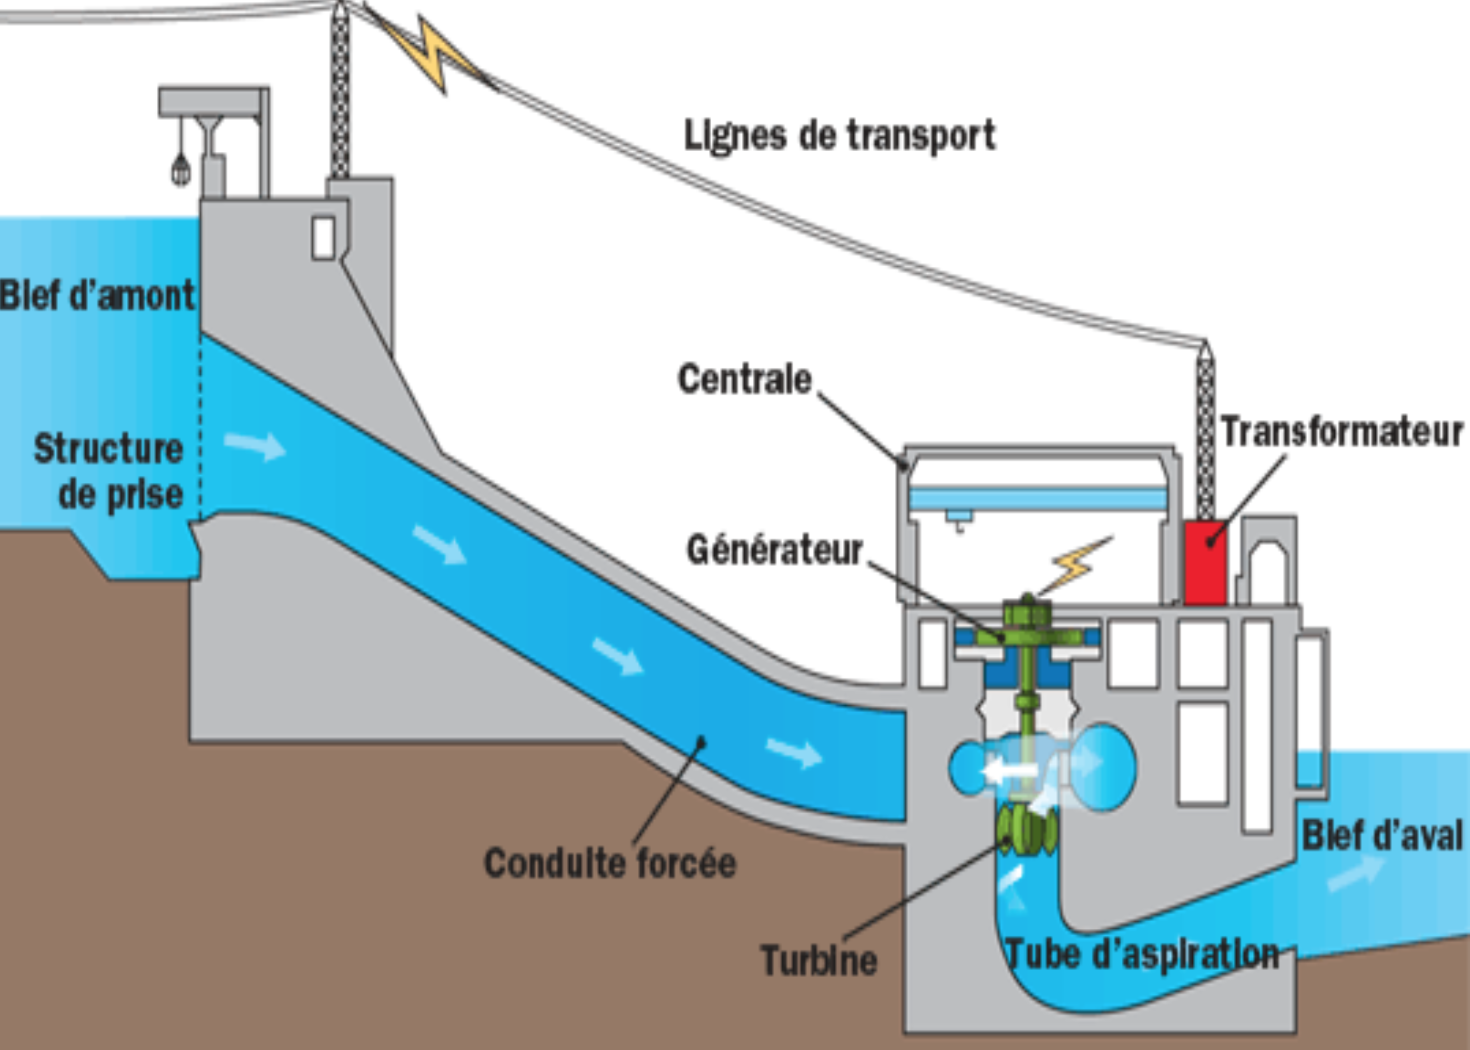
\includegraphics[scale=0.3]{ch1/2}
\captionof{figure}{}
\label{ch1/2}
\end{wrapfigure}
The major types of machine have an axial configuration so that the particles flows parallel to the shaft, radial configuration where flows enters horizontal and leaves vertical also exists. Most turbines or compressors are axial turbines. Turbopumps are most of the time radial, centrifugal. Several disks can be mounted on a same shaft (or several shafts), with fixed components changing the direction of the flow (multistage pump on \autoref{ch1/2}).

\subsection{Notations}
On \autoref{ch1/1}, 0 is the inlet of the distributor, 1 the inlet of the rotor, 2 outlet of the rotor, 3 outlet of the diffuser and i (or e)/o (or s) the upstream/downstream plenum. There are 3 velocity components: the absolute velocity $\bar{v}$, the frame tangential velocity $\bar{u}$ and the relative velocity $\bar{w}$ due to the rotation of fluid particles. 

\subsection{Velocity triangle}
\wrapfig{8}{r}{3.5}{0.3}{ch1/3}
The absolute velocity respects: 

\begin{equation}
\bar{v} = \bar{u} + \bar{w}.
\end{equation}

By defining $\alpha$ and $\beta$ the angle between $\bar{u}$ and respectively $\bar{v}$ and $\bar{w}$, we can write: 

\begin{equation}
v \cos \alpha = u + w\cos \beta \qquad w^2 = u^2 + v^2 - 2uv\cos \alpha
\end{equation}

The velocity triangle is the keypoint of a turbomachine, we have to play with the velocities by means of the mass flow rate $\dot{m}$ and the machine rpm $N$. It is important to see that these parameters are linked to the velocity triangle, for the mass flow for example $\dot{m} = \rho u A$. 


\section{Fundamental equations of the flow}
\subsection{Equations of the flow in a fixed frame}
For all developments, only \textbf{steady state} regime is considered, so that $\omega = cst$ and the flow properties are not time dependent. Moreover, boundary layers are neglected and the flow propagates in parallel slices. 

\subsubsection{Energy equation}
Let's consider sections $A_0$ and $A_1$ denoting the input and output of a non interrupted flow section, for instance 0 to 1 in previous figure. The total energy equation is: 

\begin{equation}
q = h_1 - h_0 + \frac{v_1^2 - v_0^2}{2} + g(z_1-z_0)
\label{2.1}
\end{equation}

where $q$ is the heat exchanged with the outside [J/kg], $v$ is the absolute velocity [m/s] and $h$ is the enthalpy [J/kg]. In adiabatic systems $q=0$. We see that if there is thermal, kinetic or potential energy loss, it will produce heat. Be careful that this equation is not applicable around the blade. 

\subsubsection{Equation of kinetic energy}
We know that kinetic and potential energy can be transformed into work in a machine. We have:

\begin{equation}
 \frac{v_1^2 - v_0^2}{2} + g(z_1-z_0) = - \int _{p_0}^{p_1} \nu dp - w'_f
 \label{2.2}
\end{equation}

where $\nu = 1/\rho$ is the specific volume [$m^3$/kg] and $w'_f$ the work resulting from all friction effects [J/kg]. We see that if velocity increases/decreases, pressure decreases/increases and the friction is a loss, so "-" signs. 

\subsubsection{Global thermodynamic equation}
By considering \eqref{2.2} in \eqref{2.1}: 

\begin{equation}
q + w'_f = h_1 - h_0  - \int _{p_0}^{p_1} \nu dp
\end{equation}

The physical content is different, we see that in fact the losses corresponds to pressure and temperature losses. 

\subsubsection{Mass flow rate equation}
The mass flow is constant over a tube: 

\begin{equation}
\dot{m} = \rho v A = \rho_0 v_0 A_0 = \rho_1 v_1 A_1 = \frac{v_1 A_1}{\nu _1}  
\end{equation}

where $\dot{m}$ [kg/s].

\subsection{Equations of the flow in a moving frame}
Now we can consider the indices 1 and 2 referring to the blade space. 

\subsubsection{Equation of kinetic energy in a relative space}
He skipped the long demo page 8. The equations are the same as before, the only difference is that we replace the absolute velocity by the relative one and an additional kinetic energy term due to the rotation of the frame: 

\begin{equation}
 \frac{w_2^2 - w_1^2}{2} + g(z_2-z_1) = - \int _{p_1}^{p_2} \nu dp - w^"_f + \frac{u_2^2-u_1^2}{2}
 \label{2.5}
\end{equation}

Remark that this term can play a huge role because in a centrifugal system the term is non zero while it is zero in an axial system. 

\subsubsection{Global thermodynamic equation}
The equation is exactly the same as before, except $w'_f$ that becomes $w^"_f$. 
\begin{equation}
q + w^"_f = h_2 - h_1 - \int _{p_1}^{p_2} \nu dp
\end{equation}

\subsubsection{Energy equation}
If we combine the two previous equation we get: 

\begin{equation}
q + \frac{u_2^2-u_1^2}{2} = h_2 - h_1 + \frac{w_2^2 - w_1^2}{2} + g(z_2-z_1)
\end{equation}

\subsubsection{Mass flow equation rate equation}
For a section normal to the relative velocity:

\begin{equation}
\dot{m} = \rho w A = \rho _1 w_1 A_1 = \rho _2 w_2 A_2
\end{equation}


\section{Fundamental equations of turbomachinery}
\subsection{Compressors}
\subsubsection{Internal losses}
\wrapfig{8}{l}{5}{0.3}{ch1/4}
Several kind of losses are present in a compressor. First of all, friction in the distributor gives birth to losses noted $w'_f$. Then, the fluid goes through the interblade channel where its energy increases, but a loss due to friction is present $w^"_f$. In addition, the clearance between the blade tip and the carter is non zero and leads to back-flow leakage $\dot{m}_i$ as the pressure upstream is lower. If we denote the mass flow rate through the blades $\dot{m}_R$, we have: 

\begin{equation}
\dot{m}_R = \dot{m} + \dot{m}_i
\end{equation}

A big part of the flow goes then through the diffuser, but a small part escapes from the seal to the outside $\dot{m}_e$. The small gap between the rotor and the internal carter is filled with part of the fluid. Even if this fluid does not contribute to the energy exchanges (stagnation), part of the power supplied to the shaft will dissipate due to fluid friction $P_{fr}$. 

\subsubsection{External losses}
As discussed, part of the flow escapes through the seals. The upstream one is not a problem since the pressure is close to the atmospheric pressure, but for the downstream seal $\dot{m}_e \neq 0$ since the pressure is higher. This will be neglected in the study. The last losses are due to bearings and other mechanical components such as the fuel pump that we all denote in a single absorbed power $P_{fa}$. 

\subsubsection{Energy equation}
\wrapfig{10}{l}{6.5}{0.3}{ch1/7}
Before going through all the losses appearing in the engine, let's have a global view limiting the study region as on the figure. The total energy equation between input and output is: 

\begin{equation}
q + W_{e\rightarrow s} = u_o - u_i + \frac{v_o ^2 - v_i^2}{2} + g(z_o - z_i)
\end{equation}

where we have the heat exchanged with the outside, the work from external forces to the system due to fluid pressure $p_i \nu _i - p_o\nu_o$ and work applied on the shaft $\frac{P - P_{fa}}{\dot{m}} =  \frac{P_i}{\dot{m}}$ equal to the variation of internal energy, kinetic energy and potential energy. Heat exchanges and the height difference in such engine are negligible, by introducing the enthalpy instead of internal energy and fluid pressure, we have: 

\begin{equation}
P_i = P - P_{fa} = \dot{m}\left( h_o - h_i + \frac{v_o^2 - v_i^2}{2} \right) = \dot{m} (h_{t_o} - h_{t_i}) = \dot{m} c_p (T_{t_o} - T_{t_i})
\end{equation}

where the index $t$ denotes the total or stagnation quantities. We conclude that the work transferred through the shaft increases the total energy of the fluid. 

\subsubsection{Equation of kinetic energy}
This adapted to the work $\frac{P_i}{\dot{m}}$ gives: 

\begin{equation}
P_i = \dot{m} \underbrace{\left( \frac{v_o^2-v_i^2}{2} + \int _{i}^{o} \nu dp + g(z_o - z_i)\right)}_{e} + P_f = \dot{m} e + P_f
\end{equation}

$P_f$ is the internal friction loss with the active as well as the non-active fluid and $e$ is the energy transferred to the fluid. 

\subsubsection{A first distribution of the power - efficiencies}
\wrapfig{7}{r}{3.2}{0.3}{ch1/8}
The figure summarizes all the above equations, for the efficiency we have $\dot{m}e$ at the end and we inject $P$ so: 

\begin{equation}
\eta _{g} = \frac{\dot{m}e}{P} = \frac{\dot{m}e}{P_i} \frac{P_i}{P} = \eta _i \eta _m
\end{equation}

that we rewrite as internal efficiency and external mechanical efficiency. 

\subsubsection{Energy transfer to the rotor}
The only new equation we have is the \textbf{Euler-Rateau equation}. The energy given to the flow in a pump is linked to the energy provided to the shaft. We have to consider the kinetic moment (moment of the quantity of movement) related to the shaft:

\begin{equation}
\frac{d}{dt}\sum M_{axe} (m\bar{v}) = \sum M_{axe}\bar{F}_e
\label{3.2}
\end{equation}

\wrapfig{11}{l}{3}{0.3}{ch1/5}
The variation of the kinetic moment of the rotor is zero since the rotation speed is constant. For a fluid element with mass $m$ and at a distance $r$ of the shaft, the velocity $\bar{v}$ is composed of a component // to the shaft, radial component and tangential component on the rotor. Only the tangential component delivers a moment: 

\begin{equation}
M_{axe}(m\bar{v}) = m r v \cos \alpha 
\end{equation}

and since the flow is permanent, after a time $dt$ very small, if the mass flow is constant: 

\begin{equation}
\sum _{b'b^"} mr v \cos \alpha - \sum _{a'a^"} mr v \cos \alpha = m' (r_2v_2\cos \alpha _2-r_1v_1\cos \alpha _1) = m' (r_2 v_{2u} - r_1 v_{1u})
\end{equation}

Accepting $r_2 v_{2u} - r_1 v_{1u} = cst$ for all channels we get: 

\begin{equation}
\frac{d}{dt}\sum M_{axe}(m\bar{v}) = \frac{d}{dt}\left[(r_2 v_{2u} - r_1 v_{1u}) \sum m'\right] = \dot{m}_R (r_2 v_{2u} - r_1 v_{1u})
\end{equation}

For the right hand side of \eqref{3.2}, the weight of the wheel, the weight of the fluid, the pressures at inlet, at outlet and at side walls are null due to symmetry. Only the \textbf{driving torque} applied on the shaft $\bf{M_i}$ and the \textbf{resistive torque} $-\bf{M_{fr}}$ due to friction between the wheel and the non-active fluid are present, so that we finally get: 

\begin{equation}
\dot{m}_R (r_2 v_{2u} - r_1 v_{1u}) = M_i - M_{fr}
\end{equation}

And if we multiply by $\omega$: 

\begin{center}
\theor{
\textbf{Equation of Euler-Rateau}
\begin{equation}
P_i - P_{fr} = P - P_{fa} - P_{fr} = P_R = \dot{m}_R (u_2 v_{2u} - u_1 v_{1u}) = \dot{m}_R \Delta (uv_u)
\end{equation}
This equation tells that in order to be transferred to the mass flow rate $\dot{m}_R$, the power at the rotor shaft $P_R$ must show an increase of the quantity $uv_u$ which is directly related to the velocity triangle. 
}
\end{center}

As $w^2 = v^2 + u^2 - 2 u v_u$, one can also write: 

\begin{equation}
P_R = \dot{m}_R \left( \frac{v_2 ^2 - v_1^2}{2} + \frac{u_2 ^2 - u_1^2}{2} - \frac{w_2 ^2 - w_1^2}{2} \right)
\label{3.8}
\end{equation}

\subsubsection{Energy generated by the rotor}
Remember \eqref{2.5} and replace this in \eqref{3.8}, we get: 

\begin{equation}
P_R = \dot{m}_R \underbrace{\left( \frac{v_2 ^2 - v_1^2}{2}  + \int _{p_1}^{p_2} \nu dp + g(z_2 - z_1) \right)}_{e_R} + \dot{m} _R w^"_f
\end{equation}

where $e_R$ is the energy transferred to the fluid through the channels on the rotor between section 1 and 2 on the common figure. $\dot{m}_R w^"_f = P^"_f$ being the power absorbed by friction effects, we get: 

\begin{center}
\theor{
\begin{equation}
P_R = \dot{m}_Re_R + P^"_f \qquad \left(\mbox{and } P_R = \dot{m} (h_{t_2} - h_{t_1}) \right)
\end{equation}
}
\end{center}

And we get thus 4 different expression for $P_R$, where the last expression was given in lecture. 

\subsection{Detailed power distribution}
The different losses can be depicted thanks to the previous equation:

\begin{equation}
P_i = P-P_{fa} \qquad P_R = P_i - P_{fr} \qquad \dot{m}_Re_R = P_R - P^"_{f} \qquad \dot{m}_R = \dot{m} + \dot{m}_i
\end{equation}

\wrapfig{12}{l}{5}{0.3}{ch1/6}
where we clearly see the mechanical losses, the loss due to stationary fluid, the loss at the rotor and the back flow. To this we have to add the loss at the diffuser and distributor which we wrote as:

\begin{equation}
P'_f = \dot{m}w'_f
\end{equation}

On the figure, we first see the loss due to mechanical components giving $P_i$, then the fluid losses composed of stationary fluid losses giving $P_R$, then rotor channels loss giving $\dot{m}_Re_R$, but we have the back flow loss $\dot{m}_i e_R$ giving $\dot{m}e_R$ and the last venturi losses that gives the output power $\dot{m}e$ plus all the losses. 

\section{Turbines}
\subsubsection{Description}
\wrapfig{11}{r}{4.5}{0.3}{ch1/9}
The equations are in fact the same except that we have to adapt the signs and indexes to the working principle since the energy is flowing from the fluid to the shaft. As before, there is a clearance flow $\dot{m}_i$ such that: 

\begin{equation}
\dot{m} = \dot{m}_R + \dot{m}_i
\end{equation}

The losses due to mechanical components $P_{fa}$ and the leakage flows $\dot{m}_e$ (negligible), the energy losses in non rotating ($w'_f$) and rotating ($w^"_f$) frame and the loss due to non-active fluid $P_{fr}$ are present. The useful power $P_u$ replaces the $P$ we had before. 

\subsubsection{Energy equation}
It is the same as before except that the indexes are inverted and the useful power is $P_u = P_i - P_{fa}$:

\begin{equation}
P_i = P_u + P_{fa} = \dot{m} (h_{t_i} - h_{t_o})
\end{equation} 

\subsubsection{Equation of kinetic energy}
\begin{equation}
P_i = \dot{m} \underbrace{\left( \frac{v_i^2-v_o^2}{2} + \int _{p_o}^{p_i} \nu dp + g(z_i - z_o)\right)}_{e} - P_f = \dot{m} e - P_f
\end{equation}

\subsubsection{First distribution of the power}
The efficiencies are inverted: 

\begin{equation}
\eta _g = \frac{P_u}{\dot{m}e} = \frac{P_u}{P_i}\frac{P_i}{\dot{m}e} = \eta _m \eta _i
\end{equation}

On \autoref{ch1/10} is represented a first plot of the different powers, remark that it is similar to what we had, only the fluid losses comes before the mechanical losses. The fluid losses are the same as before. 

\minifig{ch1/10}{ch1/11}{0.4}{0.27}{0.35}{0.35}

\subsubsection{Equation of Euler-Rateau}
We can rewrite $P_R$ as the power transfered to the rotor from the fluid $\dot{m}_R$: 

\begin{equation}
P_R = P_i + P_{fr} = \dot{m} _R (u_1v_1\cos \alpha _1 - u_2v_2\cos \alpha _2) 
\end{equation}

\subsubsection{Energy absorbed by the rotor}
As before, combing the above equation and the equation for rotating frame we get: 

\begin{equation}
P_R = \dot{m}_R e_R - P^"_f
\end{equation}


\section{Axial thrust and disc friction}
\subsection{Definition}
Since turbomachines are used to increase the energy of the fluid or extract energy from it, the pressure at the two sides of the rotor is different. This leads to an axial force and we need \textbf{thrust bearings} to avoid the shaft to slip. 

\subsection{Equation of the axial thrust}
\wrapfig{9}{l}{3.5}{0.3}{ch1/12}
We apply the equation of quantity of movements to the wheel and fluid without the shaft between section 1 and 2: 

\begin{equation}
\sum \frac{d}{dt}(m\bar{v}) = \sum \bar{F}_e
\end{equation}

We will make a projection along x-axis. The present external forces are: pressure forces $p_1A_{R1}$ and $p_2A_{R2}$, weight of the rotor and the fluid projected is $G\cos \delta$ and reaction force of the shaft on the rotor with projection $F_{ax}$ so $-F_{ax}$ as seen by the rotor (projection of moments is null). The equation of quantity of movement becomes: 

\begin{equation}
\begin{aligned}
&\dot{m}_R\, (v_{2ax} - v_{1ax}) = p_1 A_{R1} - p_2 A_{R2} + F_{ax} + G\cos \delta \\
\Leftrightarrow\qquad &F_{ax} = \dot{m}_R\, dt (v_{2ax} - v_{1ax}) + P_2 A_{R2} - P_1 A_{R1} -  G\cos \delta
\end{aligned}
\end{equation}

\subsection{Friction of the disc}
\wrapfig{9}{l}{5.5}{0.3}{ch1/13}
As mentioned before, there is friction between the disc and the non-active fluid. It is obvious that the friction torque will increase with the radius (more surface), the rpm ($u$) and the volumetric mass of the fluid. Considering an elementary surface $2\pi r\, dr$, we find experimentally for the elementary friction force and torque: 

\begin{equation}
dF_{fr} = K\rho u^2 2\pi r \,dr \qquad dC_{fr} = 2K\rho 2\pi r^2\, dr\, u^2 
\end{equation}

the 2 appears by considering the 2 sides of the disc. We integrate from internal radius $r$ to the external one $r_1$ and multiply by $\omega$ to have powers (neglect $r^5$ compared to $r_1^5$): 

\begin{equation}
C_{fr} = K\rho \omega ^2 r_1^5 \qquad \Rightarrow P_{fr}= K\rho \omega ^3 r_1^5
\end{equation}

Remark that one could think that we will have enormous values for $\omega ^3$, but be aware that if $\omega$ increases, the mechanical stresses on the device increases and force to reduce the $r_1$. This is why the friction is finite. If the side walls are very smooth, the coefficient K is related to the Reynolds number: 

\begin{equation}
Re = \frac{\rho \omega r_1^2}{\mu}
\end{equation}


\chapter{Interaction matière-lumière}
\section{Équations de Maxwell}
Les équations de \textsc{Maxwell} du champ électrique et du champ d'induction magnétique sont 
désormais bien connue
\begin{equation}
{\bf E} ({\bf r},t) = - \mbox{\boldmath $ \nabla $} \Phi({\bf r},t) - 
  \frac{\partial }{\partial t} {\bf A} ({\bf r},t),\qquad\qquad
  {\bf B} ({\bf r},t) = \mbox{\boldmath $ \nabla $} \times {\bf A} ({\bf r},t)
\end{equation}
La jauge de \textsc{Coulomb} $\vec\nabla.\vec{A}=0$ permet d'imposer des ondes transverses. On obtient
alors l'équation d'onde
\begin{equation}
\nabla ^2 {\bf A} - \frac{1}{c^2} \frac{\partial ^2 {\bf A}}{\partial t ^2} = 0 
\end{equation}
Nous avons en effet $\phi=0$ dans le vide. La solution de cette équation est une onde plane
monochromatique
\begin{equation}
{\bf A}(\omega; {\bf r},t) = {\bf A}_0(\omega) 
   \cos ( {\bf k} \cdot {\bf r} - \omega t  
 + \delta_{\omega} ) 
\end{equation}
où $\vec A_0$ est le vecteur d'amplitude, qui décrit l'intensité et la polarisation de la radiation, $\vec{k}$ est le vecteur de 
propagation ($\omega=kc$) et où $\delta_\omega$ est une phase réelle. Comme annoncé, la jauge de
\textsc{Coulomb} impose
\begin{equation}
\mbox{\boldmath $ \nabla $} \cdot {\bf A} = 0  \; \; \mbox{si} \; \; 
   {\bf k} \cdot {\bf A}_0(\omega) = 0 
\end{equation}
Les ondes sont donc transverses : $\vec{k}\perp\vec{A_0}(\omega)$. Avec ce choix de potentiel vecteur,
nous pouvons ré-écrire le champ électrique, l'induction magnétique 
\begin{equation}
{\bf E} ({\bf r},t)  = E_0(\omega)
\hat{ \mbox{\boldmath $ \epsilon $} } 
  \; \sin ( {\bf k} \cdot {\bf r} - \omega t + \delta_{\omega}),\qquad\qquad
  {\bf B} ({\bf r},t) = E_0(\omega)
\omega^{-1}
 ({\bf k} \times \hat{ \mbox{\boldmath $ \epsilon $}} )
\; \sin ( {\bf k} \cdot {\bf r} - \omega t + \delta_{\omega})
\end{equation}
et le potentiel vecteur
\begin{equation}
 {\bf A}_0(\omega) = A_0(\omega) 
\hat{  \mbox{\boldmath $ \epsilon $}}
\Rightarrow   {\bf k} \cdot 
\hat{  \mbox{\boldmath $ \epsilon $}} = 0
\end{equation}
où $\vec{\hat{\epsilon}}$ est le vecteur de polarisation. Il nous informe la direction dans laquelle
$\vec{A_0}$ pointe. Comme $\vec{E}$ contient également ce vecteur, il est forcément colinéaire à 
$\vec{A_0}$. L'onde est forcément transverse ($\vec{k}\perp\vec{A}$) et la direction de polarisation
de $\vec{E}$ est imposée par $\vec{A}$. Notons qu'il est possible de déterminer un état arbitraire
de polarisation en effectuant la combinaison de deux ondes planes indépendantes. Notons également
que $E_0(\omega) = - \omega A_0(\omega)$.\\

A l'aide du vecteur de \textsc{Poynting} ($\propto |E|^2$), il est possible de déterminer l'intensité
du champ électrique (ou du potentiel vecteur)
\begin{equation}
  I(\omega) 
= \frac{1}{2} \epsilon_0 c E_0^2 (\omega) 
=  \frac{1}{2} \epsilon_0 c \omega^2  A_0^2 (\omega) 
= \frac{\hbar \omega N(\omega) c}{V}
= \rho (\omega) c
\end{equation}
La dernière égalité est le produit de la densité photonique par la vitesse de la lumière. La densité
photonique (ou densité de radiation) s'exprime
\begin{equation}
\rho(\omega) 
= \frac{1}{2} \epsilon_0 E_0^2 (\omega)
= \frac{1}{2} \epsilon_0 \omega^2
A_0^2 (\omega) = \frac{N (\omega) \hbar \omega}{V}
\end{equation}
Cette densité est l'énergie $\hbar\omega$ que porte chaque photon, multiplié par $N(\omega)$ le nombre
de photon, par la vitesse de la lumière $c$ et divisé par le volume. Il s'agit bien d'une énergie par
unité de surface et de temps.\\

Notons les deux relations intégrales suivantes
\begin{equation}
I = \int_0^\infty I (\omega) d\omega \hspace*{1cm};
\hspace*{1cm}
\rho = \int_0^\infty \rho (\omega) d\omega 
\end{equation}
Ces relations sont rencontrée lorsque l'on ne se situe pas dans un cas monochromatique : par exemple,
un \textit{pulse} a une forme dans l'espace et le temps.

\section{Équation de Schrödinger dépendante du temps}
Les solutions des équations de \textsc{Maxwell} pouvant bien évidemment dépendre du temps, il faut se
soucier de l'évolution dans le temps (mais aussi toujours de l'espace) du potentiel vecteur en tenant
compte du fait que ce n'est pas intégralement monochromatique. On défini alors la forme générale d'un
pulse de radiation
\begin{equation}
  {\bf A} ({\bf r}, t) 
= \hat{  \mbox{\boldmath $ \epsilon $}}
\int_{\Delta \omega} A_0 (\omega) 
   \cos ( {\bf k} \cdot {\bf r} - \omega t + 
\delta_{\omega} )  \; d \omega
\end{equation}
L'hamiltonien d'une particule chargée (sans spin) dans un champ électromagnétique s'écrit
\begin{equation}
H = \frac{1}{2m} ({\bf p} - q {\bf A} ) ^2 + q \Phi
\end{equation}
Utilisons celui-ci pour écrire l'équation de Schrödinger dépendante du temps
\begin{equation}
i \hbar \frac{\partial}{\partial t} \Psi ({\bf r}, t)
= \left[ \frac{1}{2m} (-i \hbar  \mbox{\boldmath $ \nabla $} + e {\bf A}) ^2
  - \frac{Ze^2}{(4 \pi \epsilon_0) r } \right] \Psi ({\bf r}, t)
\end{equation}
Comme $\vec\grad A=0$ (jauge de \textsc{Coulomb}), nous avons que
\begin{equation}
 \mbox{\boldmath $ \nabla $} \cdot ({\bf A} \Psi )
= {\bf A} \cdot (  \mbox{\boldmath $ \nabla $} \Psi)
\end{equation}
Il est donc possible de remplacer le double produit par l'un de ces deux termes. A un facteur 2 près,
ça n'a pas d'importance. Ce facteur disparait d'ailleurs dans la forme réécrite ci-dessous
\begin{equation}
i \hbar \frac{\partial}{\partial t} \Psi ({\bf r}, t) =\left[ -\frac{\hbar ^2}{2m} \nabla ^2 - \frac{Ze^2}{(4 \pi \epsilon_0) r } 
  - \underbrace{\frac{i \hbar e}{m} {\bf A} \cdot \mbox{\boldmath $ \nabla $} 
  + \frac{e^2}{2m} {\bf A} ^2}_{(*)} \right] \Psi ({\bf r}, t)
\end{equation}
La ré-écriture fait apparaitre deux termes (marqués par $(*)$) dans l'Hamiltonien. Ceux-ci sont 
négligeable, il est nécessaire que l'intensité soit faible (car $I = f(\vec{A})$).\\

On peut considérer que l'on se trouve dans un cas de champs faibles si
\begin{equation}
  {\bf A}^2 \ll {\bf A}
\end{equation}
L'exclusion des termes en $A^2$ signifie que l'on est contraint de considérer le cas ou nous avons
l'émission ou l'absorption d'un seul photon à la fois (le bas bi-photonique ne peut pas être traité
sous cette hypothèse). Sous celle-ci, l'équation de Schrödinger dépendante du temps s'écrit plus
simplement
\begin{equation}
i \hbar \frac{\partial}{\partial t} \Psi  = [ H_0 + H'(t)] \Psi
\end{equation}
où $\DS H_0 = -\frac{\hbar ^2}{2m} \nabla ^2 - \frac{Ze^2}{(4 \pi \epsilon_0) r }$ et 
$\DS H'(t) = - \frac{i \hbar e}{m} {\bf A} \cdot \mbox{\boldmath $ \nabla $}$.\\

Pour résoudre cette équation, nous allons introduire la \textit{théorie des perturbations dépendantes
du temps}. Supposons que l'on ai résolu le problème aux valeurs propres $H_0 \psi_k = E_k \psi_k$. 
Nous pouvons alors écrire 
\begin{equation}
\Psi = \sum_k c_k(t) \psi_k ({\bf r}) e^{-iE_kt/\hbar}
\end{equation}
En insérant cette équation dans celle de Schrödinger écrite ci-dessus, on trouve l'expression 
analytique exacte suivante
\begin{equation}
 \dot{c}_b(t) = \frac{1}{i \hbar} \sum_k H'_{bk} (t) c_k (t) e^{i \omega_{bk} t }
\end{equation}
Pour que cette expression ai un sens, il faut que $H'$ puisse couplet l'état $n$ et l'état $k$ sur
lequel porte la somme afin d'avoir un transfert de population d'n état non-perturbé vers une somme
d'états perturbés
\begin{equation}
 H'_{bk} (t) = \langle \psi_b \vert H'(t) \vert \psi_k \rangle,\qquad\qquad
 \omega_{bk} = (E_b - E_k) / \hbar
\end{equation}
La perturbation va donc peupler d'autres état par implication même de cette perturbation.\\

Hélas, cette équation \textit{exacte} n'est pas ré-solvable. Il est nécessaire d'introduire une 
condition initiale stipulant qu'initialement, le seul état peuplé est $a$
\begin{equation}
\Psi (t=0) = \psi_a  \Rightarrow  c_k (t \leq 0) = \delta_{ka} 
\end{equation}
La théorie des perturbations à l'ordre un nous donne
\begin{equation}
c_b^{(1)} (t) = \frac{1}{i \hbar} \int_0^t H'_{ba}(t') e^{i \omega_{ba} t' } dt'
= -\frac{e}{m} \int_0^t 
   \langle \psi_b \vert {\bf A} \cdot \mbox{\boldmath $ \nabla $}  \vert \psi_a \rangle
   e^{i \omega_{ba} t' } dt'
\end{equation}
Le potentiel vecteur est lui donné par
\begin{equation}
  {\bf A} ({\bf r}, t) 
= \hat{  \mbox{\boldmath $ \epsilon $}}
\int_0^\infty A_0 (\omega) 
   \cos ( {\bf k} \cdot {\bf r} - \omega t + 
\delta_{\omega} )  \; d \omega
\end{equation}
où $\omega$ est la fréquence atomique. En substituant cette expression
\begin{equation}
\begin{array}{ll}
 c_b^{(1)} (t) = \DS&\DS-\frac{e}{2m} 
\int_0^\infty d\omega A_0(\omega)\times \left[ e^{i \delta_{\omega}} 
  \langle \psi_b \vert e^{i {\bf k} \cdot {\bf r} }
  \hat{  \mbox{\boldmath $ \epsilon $}} \cdot \mbox{\boldmath $ \nabla $}
  \vert \psi_a \rangle \int_0^t dt' e^{i(\omega_{ba} - \omega) t' } \right.\vspace{2mm}\\
\DS    &\DS+\left. e^{-i \delta_{\omega}} 
  \langle \psi_b \vert e^{-i {\bf k} \cdot {\bf r} }
  \hat{  \mbox{\boldmath $ \epsilon $}} \cdot \mbox{\boldmath $ \nabla $}
  \vert \psi_a \rangle \int_0^t dt' e^{i(\omega_{ba} + \omega) t'} \right]
\end{array}
\end{equation}
où $|c_b^{(1)}|^2$ est la probabilité de trouver $\omega=\omega_{ba}$, $\omega=-\omega_{ba}$ ou
les deux. Nous voyons apparaître un terme de phase où l'on retrouve dans les termes de phase la
fréquence de l'opérateur $\omega$ (fréquence atomique) mais aussi $\omega_{ba} = \omega_b-\omega_a$
(soit une "différence d'énergie") qui peut être négative.\\

Globalement, il existe deux possibilités : $\omega=\omega_{ba}$ ou $\omega=-\omega_{ba}$. En fonction
de la possibilité, un des deux termes "entre crochet" va s'annuler\footnote{En réalité, en prenant 
le module carré, il y aura un terme d'interférences. On peut montrer que celui-ci est  négligeable, 
nous ne le prendrons pas en compte}.\\

\cadre{\begin{description}
\item[Absorption] La première intégrale sur $t'$ est négligeable, sauf si
\begin{equation}
 \omega_{ba} \approx \omega \rightarrow E_b \approx E_a + \hbar \omega
\end{equation} 
\item[Émission] La seconde intégrale sur $t'$ est négligeable, sauf si
\begin{equation}
\omega_{ba} \approx - \omega \rightarrow E_b \approx E_a - \hbar \omega
\end{equation}
\end{description}}\ \\

Il s'agit de deux phénomènes stimulés, nous aurons l'occasion d'en reparler. La première 
condition $\omega = \omega_{ba}$ est la \textit{condition de résonance de Bohr} : il faut que
le photon ai juste l'énergie entre les deux états pour que ça puisse se produire. Savoir quel terme
"survit" c'est bien, mais il reste à calculer l'intégrale.\\

Afin de ne pas faire de recopiage inutile, renommons l'élément de matrice
\begin{equation}
M_{ba} \equiv  \langle \psi_b \vert e^{i {\bf k} \cdot {\bf r} }
  \hat{  \mbox{\boldmath $ \epsilon $}} \cdot \mbox{\boldmath $ \nabla $} \vert \psi_a \rangle
\end{equation}
Il s'agit en réalité de l'\textit{élément de couplage}. Sous cette notation, le module carre discuté
ci-dessus s'écrit
\begin{equation}
  \vert c_b^{(1)} (t) \vert ^2 = \frac{1}{2}
\left( \frac{e}{m} \right) ^2
 \int_0^\infty d \omega
  A_0 (\omega) ^2
    \vert M_{ba} (\omega) \vert ^2 \; F(t,\omega - \omega_{ba} )
\end{equation}
où $A_0$ est une amplitude proportionnelle à l'intensité du champ et $F$ est une fonction dépendante
du temps $t$
\begin{equation}
F(t,\tilde{\omega}) \equiv F(t,\omega - \omega_{ba}) 
= \frac{1 - \cos \tilde{\omega} t }{\tilde{\omega}^2}
\end{equation}
Le résultat de l'intégrale de $F$ est bien connu
\begin{equation}
\int_{-\infty}^{+\infty}
F(t, \tilde{\omega}) d\tilde{\omega} = t 
\int_{-\infty}^{+\infty} \frac{\sin^2 x }{x^2} dx = \pi t
\end{equation}

	\begin{wrapfigure}[10]{r}{5cm}
	\vspace{-5mm}
	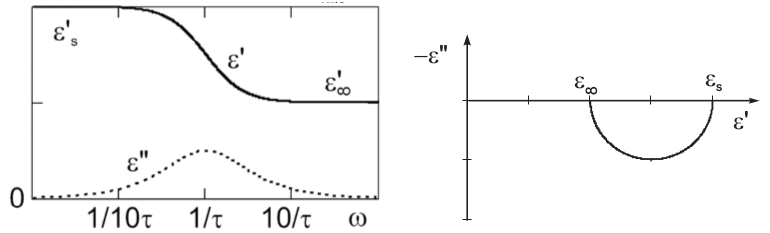
\includegraphics[scale=0.4]{ch2/image1}
	\captionof{figure}{ }
	\end{wrapfigure}
Ci-contre, une représentation de $F(t,\tilde{\omega})$. Il ne s'agit pas d'un delta de \textsc{Dirac}.
Par contre, sous l'approximation du temps long, la largeur du pulse devient suffisamment mince que
pour considérer que c'est le cas
\begin{equation}
F(t \rightarrow \infty, \tilde{\omega}) \sim \pi t \; \delta(\tilde{\omega})
\end{equation}
Revenons au calcul précédent en utilisant ce résultat pour l'intégration sur tous les
$\tilde{\omega}$
\begin{equation}
  \vert c_b^{(1)} (t) \vert ^2 = 
\frac{1}{2} \left( \frac{e}{m} \right) ^2
A_0^2 (\omega_{ba}) 
     \vert M_{ba} (\omega_{ba}) \vert ^2 \; 
\underbrace{\int_{-\infty}^{+\infty}
F(t, \tilde{\omega}) d \tilde{\omega}}_{\pi t}
\end{equation}
On trouve alors que la probabilité augmente \textbf{linéairement} avec $t$ \\

\cadre{\begin{equation}
\vert c_b^{(1)} (t) \vert ^2 = \frac{\pi}{2}
 \left[ \frac{e A_0 (\omega_{ba})}{m} \right] ^2
    \vert M_{ba} (\omega_{ba}) \vert ^2 \; t
\end{equation}}\ \\

Il s'agit d'une nouvelle condition de résonance nous informant sur le fait que $\omega$ doit
être proche de $\omega_{ba}$.\footnote{A vérifier.}

\section{Absorption et émission stimulées}
La probabilité d'\textbf{absorption} s'obtient en dérivant temporellement le module carré calculé 
ci-dessus
\begin{equation}
W_{b \leftarrow a} =
\frac{d}{dt} \vert c_b^{(1)} (t) \vert ^2 =
\frac{\pi}{2} \left[ \frac{e A_0 (\omega_{ba}) }{m} \right] ^2 
\vert M_{ba} (\omega_{ba}) \vert ^2
\end{equation}
En reprenant le lien entre $A_0$ est $I$ (en début de chapitre, avec le vecteur de \textsc{Poynting})
\begin{equation}
W_{b \leftarrow a} =\frac{4 \pi ^2}{m^2 c} \left( \frac{e^2}{4 \pi \epsilon_0 } \right)
\frac{I( \omega_{ba}) }{\omega_{ba}^2 } \vert M_{ba} (\omega_{ba}) \vert ^2
\end{equation}
Cette probabilité sera  non nulle lorsque l'élément matriciel $M_{ba}$ est nul nul. Ceci met en 
évidence la quantification de la matière par l'atome d'hydrogène. L'interaction lumière-matière sera
traitée de façon semi-classique. \\

Il existe un effet symétrique inverse à celui-ci : $\tilde W_{b\leftarrow a}=W_{b\leftarrow a}$. Ce
phénomène est l'\textbf{émission stimulée} dont la probabilité est donné par
\begin{equation}
\tilde{W}_{a \leftarrow b} = \frac{4 \pi ^2}{m^2 c} \left( \frac{e^2}{4 \pi \epsilon_0 } \right)
\frac{I( \omega_{ba}) }{\omega_{ba}^2 } \vert \tilde{M}_{ab} (\omega_{ba}) \vert ^2
\end{equation}
En définissant l'élément de matrice
\begin{equation}
\tilde{M}_{ab} = \langle \psi_a \vert e^{-i {\bf k} \cdot {\bf r} }
  \hat{  \mbox{\boldmath $ \epsilon $}} \cdot \mbox{\boldmath $ \nabla $} \vert \psi_b \rangle
\end{equation}
En comparant cet élément matriciel au précédent, c'est sans surprise que l'on retrouve
\begin{equation}
\tilde{M}_{ab} = - M_{ba}^{\ast} \Rightarrow \tilde{W}_{a \leftarrow b} = W_{b \leftarrow a}
\end{equation}
La seule différence par rapport au cas précédent se situe donc dans l'élément de matrice. Les 
populations $a$ et $b$ ne seront pas peuplées de la même façon. Selon \textsc{Boltzmann}, la 
population dépend de l'énergie ($N\propto g_ie^{-E/kT}$). Si l'on tient compte de ce facteur 
de proportionnalité, il y a plus de change d'observer une absorption qu'une émission stimulé. Ceci
n'est évidemment pas le cas dans des dispositifs comme les \textit{laser} où il y a eu inversion 
de la population, mais rappelons que cette situation ne décrit pas un équilibre thermodynamique.



\section{Le photon QED et l'émission spontanée}
Nous avons jusqu'ici suivi une approche semi-classique. En passant par le théorie quantique des 
champs, nous allons essayer d'estimer l'erreur faite (section informative si j'ai bien compris). 

\subsection{Absorption d'un photon à partir d'un état à $N$ photons}
En quantifiant le champ électrique, on retrouve un potentiel vecteur ayant exactement la même forme
que précédemment
\begin{equation}
  {\bf A}_1 = 
  \hat{  \mbox{\boldmath $ \epsilon $}}
\left[  \frac{2 N(\omega) \hbar}{ V \epsilon_0 \omega}
  \right] ^{1/2} \frac{1}{2}
  \exp [ i ( {\bf k} \cdot {\bf r} - \omega t 
+ \delta_{\omega} )  ] 
\end{equation}
On trouve alors la même expression qu'avant, la QED n'apporte rien ici
\begin{equation}
W_{b \leftarrow a} ^{QED} = 
W_{b \leftarrow a} 
= \frac{4 \pi ^2}{m^2 c} \left( \frac{e^2}{4 \pi \epsilon_0 } \right)
\frac{I( \omega_{ba}) }{\omega_{ba}^2 } \vert M_{ba} \vert ^2
\end{equation}


\subsection{Création d'un photon}
Par de chance cette fois-ci, le potentiel vecteur n'est pas totalement similaire
\begin{equation}
  {\bf A}_2 = 
  \hat{  \mbox{\boldmath $ \epsilon $}}
\left[ \frac{ 2(  N(\omega)+1) \hbar}{ V \epsilon_0 \omega}
  \right] ^{1/2} \frac{1}{2}
   \exp [ -i ( {\bf k} \cdot {\bf r} 
- \omega t + \delta_{\omega} ) ]
\end{equation}
La différence, c'est ce +1. Il s'agit du photon qui manque à la théorie semi-classique. Dès lors
\begin{equation}
\tilde{W}_{a \leftarrow b}^{QED} =
 \frac{4 \pi ^2}{m^2 } \left( \frac{e^2}{4 \pi \epsilon_0 } \right)
\frac{( N (\omega_{ba}) + 1) \hbar }{V \omega_{ba} } \vert M_{ba} \vert ^2
  \delta(\omega - \omega_{ba} )
\end{equation}
Rassurons-nous, c'est quasi-négligeable ($ N (\omega_{ba}) + 1 \approx N (\omega_{ba})$). On peut
alors souvent écrire, en approximation
\begin{equation}
\tilde{W}_{a \leftarrow b}^{QED} \approx
\tilde{W}_{a \leftarrow b} =  
\frac{4 \pi ^2}{m^2 c} \left( \frac{e^2}{4 \pi \epsilon_0 } \right)
\frac{I( \omega_{ba}) }{\omega_{ba}^2 } \vert \tilde{M}_{ab} \vert ^2
\end{equation}
Ceci signifie qu'un atome dans un état excité, même dans le vide le plus total, peut émettre un
photon grâce à ce "+1" (en se désexcitant).\\

En résumé, nous pouvons dire que
\begin{equation}
\left\{\begin{array}{ll}
\mbox{semi-classique:} & N(\omega_{ba}) \\
\mbox{QED:} & N(\omega_{ba}) + 1
\end{array} \right.
\end{equation}
Reprenons la précédente expression débarrassée du $N(\omega)$, soit juste le terme "+1" que nous
avions manqué dans l'approche semi-classique. Il s'agit de la \textit{probabilité d'émission
\textbf{spontanée}}
\begin{equation}
W_{a \leftarrow b}^s =
 \frac{4 \pi ^2}{m^2 } \left( \frac{e^2}{4 \pi \epsilon_0 } \right)
\frac{\hbar }{V \omega_{ba} } \vert M_{ba} \vert ^2
  \delta(\omega - \omega_{ba} )
\end{equation}
Afin d'interpréter ce terme, nous allons faire un petit détour par la \textit{Règle d'Or de Fermi}\\

\cadre{
$$\rho_b(E) \equiv~\mbox{densit\'e de niveaux}
\Rightarrow
P_{ba}(t) = \frac{2 \pi}{\hbar} \vert H'_{ba} \vert ^2
\rho_b(E) t$$
$$\mbox{prob. transition par unit\'e de tps}:~
W_{b \leftarrow a} = dP_{ba}/dt $$
$$W_{b \leftarrow a} = \frac{2 \pi}{\hbar} \vert H'_{ba} \vert ^2
\rho_b(E)$$
Il s'agit de la probabilité de passage d'un état $a$ vers un état $b$ où le passage se fait d'un
état d'énergie discret vers un état continu.}\ \\

Évaluons la densité d'états pour le photon final. Après un peu de physique du solide (en admettant
le concept de cavité de résonance)\footnote{\textit{Ceci est donné pour faire plaisir mais n'est
pas matière d'examen}}
\begin{equation}
dn_x \; dn_y \; dn_z = \left( \frac{L}{2 \pi}  \right) ^3
dk_x \; dk_y \; dk_z
 = \left( \frac{L}{2 \pi}  \right) ^3
k^2 \; dk \; d\Omega
\end{equation}
Sachant que $V=L^3$ et $w=kc$, on peut obtenir le nombre de photon compris entre $\omega$ et 
$w+d\omega$ dans un angle solide $d\Omega$
\begin{equation}
\rho_a (\omega) d \omega d \Omega = \frac{V}{(2 \pi)^3}
\frac{\omega^2}{c^3} d \omega d \Omega 
\end{equation}
En reprenant l'expression de l'émission spontanée $W^s$ et en y insérant la règle d'or de Fermi, 
on trouve
\begin{equation}
W_{a \leftarrow b}^s(\theta,\phi) d \Omega = 
\frac{\hbar}{ 2 \pi m^2 c^3} \left( \frac{e^2}{4 \pi \epsilon_0 } \right)
 \omega_{ba} \vert M_{ba} (\omega_{ba}) \vert ^2
d \Omega
\end{equation}
Ceci n'est rien autre que la probabilité d'émission \textbf{spontanée} par unité de temps d'un photon
de fréquence $\omega_{ba}$ dans une direction particulière à l'intérieur d'un angle solide $d\Omega$.


\section{L'approximation dipolaire électrique}
Lorsqu'un atome excité se désexcite par l'émission d'un photon, rien ne dit que celui-ci sera
polarisé et de même pour sa direction. Il faut alors intégrer sur tous les angles d'émission tout
en sommant sur les deux états de polarisation
\begin{equation}
W_{a \leftarrow b}^s = \frac{\hbar}{ 2 \pi m^2 c^3} \left( \frac{e^2}{4 \pi \epsilon_0 } \right)
\int d\Omega \sum_{\lambda = 1}^2 \omega_{ba} \vert M^{\lambda}_{ba} (\omega_{ba}) \vert ^2
\end{equation}
Outre cette dépendance fréquentielle, on retrouve le même élément de matrice couplant $a$ et $b$. La
question est maintenant de savoir ce que vaut cet élément de matrice et pour ça, nous allons faire
l'\textit{approximation dipolaire électrique (E1)}. Considérons le développement en série
\begin{equation}
e^{i {\bf k} \cdot {\bf r} } = 1 + (i {\bf k} \cdot {\bf r} ) + \frac{1}{2!} 
  ( i {\bf k} \cdot {\bf r} ) ^2 + \ldots
\end{equation}
Si l'on se trouve dans le cas des transitions optiques, $ \leq  1~\mbox{\AA~et }~k = 2 \pi / \lambda
\approx 10^5~\mbox{cm}^{-1}$. Il en vient que $(kr)\ll 1$. On peut approximer l'exponentielle 
à un dans ce régime la
\begin{equation}
e^{i {\bf k} \cdot {\bf r} } \approx  1  \Rightarrow
M_{ba} = \hat{  \mbox{\boldmath $ \epsilon $}} \cdot \langle \psi_b \vert
\mbox{\boldmath $ \nabla $} \vert \psi_a \rangle
\end{equation}
Il faudra alors juste calculer les éléments de matrice de l'opérateur gradient. Connaissant les 
deux relations suivantes reliant l'impulsion et la vitesse, on peut ré-écrire cet élément de 
matrice
\begin{equation}
\left.
\begin{array}{l}
{\bf p} = m \dot{{\bf r}} = -i \hbar \mbox{\boldmath $ \nabla $} \\
\dot{{\bf r}}  = \frac{1}{i \hbar} [ {\bf r}, H_0 ] \end{array}
\right\} \Rightarrow
M_{ba} = - \frac{m \omega_{ba}}{\hbar} \hat{  \mbox{\boldmath $ \epsilon $}} \cdot 
\langle \psi_b \vert {\bf r} \vert \psi_a \rangle
\end{equation}
Cette forme permet de comprendre le nom de l'approximation : on voit apparaître la position 
moyenne qui, multipliée à la charge, donne le \textit{moment dipolaire}. Sachant que
$ $, on peut écrire
\begin{equation}
W^{E1}_{b \leftarrow a} = \frac{4 \pi^2}{c \hbar^2} \left( \frac{1}{4 \pi \epsilon_0 } \right)
 I(w_{ba}) \vert  \hat{  \mbox{\boldmath $ \epsilon $}} \cdot 
 \mbox{\boldmath $ \mu $}_{ba} \vert ^2
\end{equation}
En faisant apparaître $\vec\mu$ via le formalisme position, la probabilité $E1$ permet de comprendre
le passage de $a$ à $b$ (ou l'inverse) où apparaît le moment dipolaire entre les deux états. On peut
alors trouver la radiation isotropique non polarisée pour l'absorption
\begin{equation}
W^{E1}_{b \leftarrow a} = \frac{4 \pi^2}{3 c \hbar^2} \left( \frac{1}{4 \pi \epsilon_0 } \right)
 I(w_{ba}) \vert  
 \mbox{\boldmath $ \mu $}_{ba} \vert ^2
\end{equation}
Et de même pour l'émission spontanée
\begin{equation}
W_{a \leftarrow b}^{E1,s} = \frac{4}{3 \hbar c^3} \left( \frac{1}{4 \pi \epsilon_0} \right)
  \omega_{b a}^3 \vert  \mbox{\boldmath $ \mu $}_{ba} \vert ^2
\end{equation}
On remarque que plus la différence entre $a$ et $b$ est grande, plus la probabilité de transition
est grande : c'est le \textit{comportement suicidaire de l'électron}.\\


	\begin{wrapfigure}[8]{r}{5cm}
	\vspace{-5mm}
	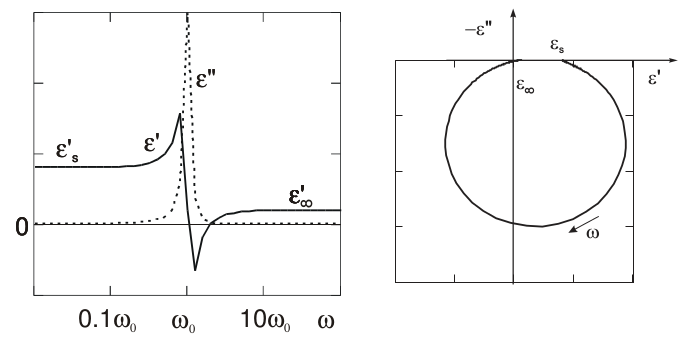
\includegraphics[scale=0.6]{ch2/image2}
	\captionof{figure}{ }
	\end{wrapfigure}
On peut (et en on parlera d'avantage dans la section suivante) faire le lien avec les coefficients
d'\textsc{Einstein}. Commentons les transitions ci-contre. Pour que la première flèche existe, il
faut que $N_a$ existe, mais également une densité de radiation $\rho$. Le coefficient $B_{ab}$ n'est
autre que le coefficient de proportionnalité donnant une probabilité. Il existe également le 
phénomène symétrique (seconde flèche) : il faut ici que $N_b$ soit peuplé et qu'il y ai une certaine
densité de radiations. La troisième flèche (émission spontanée) peut elle se produire sans radiation
à condition que le niveau $b$ soit peuplé.


\section{Lien avec les coefficients d'Einstein}
Écrivons l'équation cinétique du niveau $a$. La transition $a\to b$ dépeuple $a$ tandis que
la $b\to a$ le repeuple
\begin{equation}
\frac{dN_a}{dt} = - \frac{dN_b}{dt} =
- B_{ab} \rho(\omega_{ba}) N_a + B_{ba} \rho(\omega_{ba}) N_b
 + A_{ba} N_b
\end{equation}
A l'équilibre, $\frac{dN_a}{dt} = \frac{dN_b}{dt} = 0$. On peut en tirer un expression de $\rho$
\begin{equation}
\rho(\omega_{ba}) = 
\frac{A_{ba} }{B_{ab} (N_a/N_b) - B_{ba}}
\end{equation}
L'équation de \textsc{Boltzmann} (en oubliant les facteurs de dégénérescence) permet de déterminer
l'évolution du rapport $N_a/N_b$
\begin{equation}
\frac{N_a}{N_b} = e^{-(E_a - E_b)/kT} = e^{\hbar \omega_{ba} /kT}
\end{equation}
De son côté, \textsc{Planck} a proposé un expression pour la densité d'un corps noir
\begin{equation}
\rho(\omega_{ba})
= \frac{\hbar \omega_{ba}^3}{\pi^2 c^3}
\frac{1}{e^{\hbar \omega_{ba} /kT} -1  }
\end{equation}
\textsc{Einstein} avait les précédentes équations sous la main.  Il a remarqué - avec en plus 
l'équation de \textsc{Boltzmann} à disposition - que l'égalité entre son $\rho$ et celui trouvé par
\textsc{Planck} est vérifiée si les conditions si les conditions suivantes sont respectées
\begin{equation}
\left\{
\begin{array}{l}
B_{ab} = B_{ba} \\
A_{ba} = \frac{\hbar \omega_{ba}^3}{\pi^2 c^3} \; B_{ba}
\end{array} \right. \quad\Leftrightarrow\quad
 \left\{ \begin{array}{l}
B_{ab} = \frac{W_{b \leftarrow a}}{\rho} \\
A_{ba} = W^s_{a \leftarrow b}
\end{array} \right.
\end{equation}
\textsc{Interprétation manquante} (au pire, cf. \textit{Physique des lasers}).

\section{Spectre des atomes hydrogénoïdes}
Maintenant que nous avons établi la forme de l'élément matriciel, il serait intéressant de comprendre
comment celui-ci couple les états $n=2$ et $n=3$ par exemple. Pour se faire, reprenons la probabilité
de transition d'émission stimulée et spontanée($s$)
\begin{equation}
\begin{array}{ll}
W^{E1}_{b \leftarrow a} &\DS= \frac{4 \pi^2}{c \hbar^2} \left( \frac{e^2}{4 \pi \epsilon_0 } \right)
 I(w_{ba}) \vert  \hat{  \mbox{\boldmath $ \epsilon $}} \cdot 
{\bf  r}_{ba} \vert ^2\vspace{2mm}\\
W_{a \leftarrow b}^{E1,s}(\theta, \phi) \; d \Omega &\DS= 
\frac{1}{2 \pi \hbar c^3} \left( \frac{e^2}{4 \pi \epsilon_0} \right)
  \omega_{b a}^3
\vert  \hat{  \mbox{\boldmath $ \epsilon $}} \cdot 
{\bf  r}_{ba} \vert ^2 d \Omega
\end{array}
\end{equation}
Exprimons le vecteur polarisation $\hat{\vec{\epsilon}}$ en composantes sphériques
\begin{equation}
\left\{
\begin{array}{ll }
\epsilon^{(1)}_{+1}  & = - \frac{1}{\sqrt{2}} 
 \left( \hat{\epsilon}_x + i  \hat{\epsilon}_y \right) \\
\epsilon^{(1)}_{0}  & =  \hat{\epsilon}_z \\
\epsilon^{(1)}_{-1}  & = + \frac{1}{\sqrt{2}}
 \left(  \hat{\epsilon}_x - i  \hat{\epsilon}_y \right)
\end{array} \right.
\end{equation}
En faisant de même pour le vecteur $\vec{r}$
\begin{equation}
\left\{
\begin{array}{ll }
r^{(1)}_{+1}  & = - \frac{1}{\sqrt{2}} \left( x + i y \right) \\
r^{(1)}_{0}  & = z \\
r^{(1)}_{-1}  & = + \frac{1}{\sqrt{2}} \left( x - i y \right)
\end{array} \right.
\end{equation}
Ceci forme un tenseur sphérique irréductible d'ordre 1 (se transforme comme un vecteur par
rotation). A partir de deux tenseur, il est possible d'en tirer un tenseur scalaire. Il faut
pour cela faire un produit tensoriel des deux OTI
\begin{equation}
\left[ {\bf T}^{(k_1)} \times {\bf W}^{(k_2)} \right]^{(K)}_Q \equiv
\sum_{q_1,q_2} C(k_1k_2q_1q_2;KQ) \; T^{(k_1)}_{q_1} W^{(k_2)}_{q_2}
\end{equation}
En couplant des tenseurs sphériques irréductibles, il est possible de créer un tenseur irréductible
scalaire.

\subsubsection*{Parenthèse : symboles $3-j$}
Pour se faciliter la vie, on introduit les symboles $3-j$. Pour comprendre leur utilité, repartons
des coefficients de Clebsch-Gordon
\begin{equation}
C(j_1 j_2 m_1 m_2; J M) 
= ( j_1 j_2 m_1 m_2 \vert j_1 j_2 J M)= ( j_1 j_2 m_1 m_2 \vert  J M) 
= ( j_1 m_1 j_2 m_2 \vert  J M)
\end{equation}
Par \textbf{définition} des \textit{symboles $3-j$}
\begin{equation}
( j_1 j_2 m_1 m_2 \vert j_1 j_2 J M)
\equiv
(-1)^{j_1 - j_2 + M} [ J ]^{1/2} 
\left( \begin{array}{ccc} j_1 & j_2 & J \\ m_1 & m_2 & -M \end{array} 
\right) 
\end{equation}
L'utilité de ces symboles se trouve dans les propriétés de ceux-ci
\begin{equation}
\left( 
\begin{array}{ccc} j_1 & j_2 & j_3 \\ m_1 & m_2 & m_3 \end{array} 
\right) 
= 
\left( 
\begin{array}{ccc} j_2 & j_3 & j_1 \\ m_2 & m_3 & m_1 \end{array} 
\right)= (-1)^{j_1 + j_2 + j_3}
\left( 
\begin{array}{ccc} j_2 & j_1 & j_3 \\ m_2 & m_1 & m_3 \end{array} 
\right)
\end{equation}
Ceux-ci sont non nuls si
\begin{equation}
 \neq 0 \Rightarrow \left\{
\begin{array}{l}
\delta(j_1,j_2,j_3) \\
m_1 + m_2 + m_3 = 0
\end{array}  \right.
\end{equation}
Ce qui constitue une puissante règle de sélection.

\subsection{Produit scalaire de 2 OTI}
Construisons le produit scalaire entre deux OTI. Pour se faire, évaluons le produit entre deux
tenseurs suivant\footnote{Je n'ai pas de notes sur ce slide (20), si quelqu'un peut compléter}
\begin{equation}
\left[ T^{(k)} \times W^{(k)} \right]^{(0)}_0 \equiv
\sum_{q} 
\left( \begin{array}{ccc} k & k & 0 \\ -q & q & 0 \end{array} 
\right)  \; T^{(k)}_{-q} W^{(k)}_{q}
= (-1)^k [k]^{-1/2} \sum_q (-1)^q \; T^{(k)}_{-q} W^{(k)}_{q}
\end{equation}
On en tire l'expression du produit scalaire tensoriel\\

\cadre{
\begin{equation}
Q \equiv T^{(k)} \cdot W^{(k)} \equiv
\sum_q (-1)^q \; T^{(k)}_{-q} W^{(k)}_{q}
\end{equation}}\ \\

Nous avons comme probabilité de transition
\begin{equation}
W^{E1}_{b \leftarrow a} = \frac{4 \pi^2}{c \hbar^2} \left( \frac{e^2}{4 \pi \epsilon_0 } \right)
 I(w_{ba}) \vert  \hat{  \mbox{\boldmath $ \epsilon $}} \cdot 
{\bf  r}_{ba} \vert ^2
\end{equation}
Développons le produit scalaire se trouvant dans le module carré
\begin{equation}
\begin{array}{ll}
  \hat{  \mbox{\boldmath $ \epsilon $}} \cdot 
{\bf  r}_{ba}
&\DS= - \epsilon^{(1)}_{-1} \left( r^{(1)}_{+1} \right)_{ba} 
+ \epsilon^{(1)}_{0} \left(  r^{(1)}_{0} \right)_{ba}
- \epsilon^{(1)}_{+1}\left(  r^{(1)}_{-1} \right)_{ba}\vspace{2mm}\\
&\DS= +  \epsilon^{(1)\ast}_{+1}  \left( r^{(1)}_{+1} \right)_{ba} 
+  \epsilon^{(1)\ast}_{0}  \left(  r^{(1)}_{0} \right)_{ba}
+  \epsilon^{(1)\ast }_{-1}  \left(  r^{(1)}_{-1} \right)_{ba}\vspace{2mm}\\
&\DS= \sum_q \; \epsilon^{(1)\ast}_q I^q_{n'l'm';nlm}
\end{array}
\end{equation}
Dans l'atome d'hydrogène, $a$ et $n$ ne sont finalement qu'un \textit{set} de nombres quantiques.
Continuons en explicitant $I^q_{n'l'm';nlm}$
\begin{equation}
\begin{array}{ll}
I^q_{n'l'm';nlm} &\DS=  \sqrt{\frac{4 \pi}{3}} \int_0 ^\infty
\; dr \; r^3 R_{n'l'}(r)^\ast  R_{nl}(r)\times \int_0^{2 \pi} \int_0^{\pi}
Y^\ast_{l'm'} Y_{1q} Y_{lm} \sin \theta d\theta d\phi\vspace{2mm}\\
&\DS= \langle l' m' \vert C^{(1)}_q \vert l m  \rangle \int_0 ^\infty
\; dr \; r^3 R_{n'l'}(r)  R_{nl}(r)
\end{array}
\end{equation}
où l'on voit apparaître les harmoniques sphériques de l'opérateur. Explicitons cette fois 
$\langle l' m' \vert C^{(1)}_q \vert l m \rangle$
\begin{equation}
\langle l' m' \vert C^{(1)}_q \vert l m \rangle
= \sqrt{\frac{4 \pi}{3}} \int_0^{2 \pi} \int_0^{\pi}
Y^\ast_{l'm'} Y_{1q} Y_{lm} \sin \theta d\theta d\phi
= (-1)^{-m'} [l',l]^{1/2}
\left( \begin{array}{ccc} l' & 1 & l \\ 0 & 0 & 0 \end{array} \right)
\left( \begin{array}{ccc} l' & 1 & l \\ -m' & q & m \end{array} \right)
\end{equation}
Grâce à la propriété des coefficients $3-j$ énoncée ci-dessus, on en tire la \textbf{forte} 
règle de sélection suivante :\\

\cadre{\begin{equation}
 \neq 0 \Rightarrow \left\{
\begin{array}{l}
\delta(l',1,l) \\
(l' +1 + l)~\mbox{pair} \end{array} \right\} 
\Rightarrow \Delta l = l' - l = \pm 1
\end{equation}}\ \\

Le nombre quantique $l$ ne peut varier que d'au maximum \textbf{une} unité lors d'une transition.
On obtient finalement quelque chose de simple, à géométrie sphérique
\begin{equation}
-m' + q + m = 0 \Rightarrow
\left\{ \begin{array}{ll}
m' = m \; \; (\Delta m = 0) & \mbox{si}~q = 0 \\
m' = m \pm 1 \; \; (\Delta m = \pm 1) &\mbox{si}~q = \pm 1
\end{array} \right.
\end{equation}\ \\

A l'aide de l'explicitation de $\langle l' m' \vert C^{(1)}_q \vert l m \rangle$, on peut 
ré-écrire $I^q_{n'l'm';nlm}$
\begin{equation}
I^q_{n'l'm';nlm} =  \sqrt{\frac{4 \pi}{3}} \int_0 ^\infty
\; dr \; r^3 R_{n'l'}(r)^\ast  R_{nl}(r)\times \int_0^{2 \pi} \int_0^{\pi}
Y^\ast_{l'm'} Y_{1q} Y_{lm} \sin \theta d\theta d\phi
\end{equation}


\subsection{Lien de la règle de sélection $\Delta l = \pm 1$ avec la parité}
Nous avons
\begin{equation}
\phi_{ n l m }(r, \theta, \phi) = R_{nl} (r) Y_{lm} (\theta, \phi)
\end{equation}
A l'aide de l'opérateur parité
\begin{equation}
\hat{I} \phi_{ n l m }({\bf r}) = 
\hat{I} R_{nl} (r) Y_{lm} (\theta, \phi)
\equiv 
\phi_{ n l m }( - {\bf r})=
R_{nl} (r) Y_{lm} (\pi - \theta, \phi + \pi)
=  (-1)^l R_{nl} (r) Y_{lm} (\theta, \phi)
\end{equation}
En en tire que
\begin{equation}
\begin{array}{ll}
I^q_{n'l'm';nlm} &\DS=  (-1)^{l' + 1 + l}  I^q_{n'l'm';nlm}\\
&\DS \neq 0 ~\mbox{si}~(l' +1 + l)~\mbox{pair} 
\end{array}
\end{equation}
En résumé, l'inversion ne touche que la partie sphérique. Si $l$ est pair la parité sera impaire
et paire inversement. On en déduit qu'une\textbf{transition E1 ne peut relier que des états de
parité différentes}. La règle $\Delta l=\pm1$ est la \textit{règle de }\textsc{Laporte}. Le
\textit{slide 23} représente les transitions à l'aide de cette règle de sélection tandis que 
le \textit{slide 24} les classe par parité.


\section{Force de raie, force d'oscillateur et temps de vie}
Le théorème de \textsc{Wigner-Eckart} est apprécié pour les règles de sommes extraordinaires
des $3-j$ mais aussi pour ses règles de sélection.\\

\theor{\textsc{Wigner-Eckart}\ 
\begin{equation}
\langle \alpha j m \vert T^{(k)}_q \vert \alpha' j' m' \rangle
= (-1)^{j-m} \left( \begin{array}{ccc}
j  &  k  &  j'  \\ -m  &  q  &  m' \end{array} \right) 
\langle \alpha j \Vert {\bf T}^{(k)} \Vert \alpha' j' \rangle
\end{equation}}\ \\

Chaque élément de matrice peut s'écrire comme un élément de matrice réduit multiplié par un
$3-j$. Ré-écrivons alors l'élément de matrice qui nous intéresse sous cette forme
\begin{equation}
 \langle l m_l \vert C^{(1)}_q \vert l'm_l' \rangle =
(-1)^{l-m_l} \left( \begin{array}{ccc}
l  &  1  &  l'  \\ -m_l  &  q  &  m_l' \end{array} \right) 
\langle  l \Vert {\bf C}^{(1)} \Vert l' \rangle
\end{equation}
L'élément de matrice réduit s'écrit
\begin{equation}
\langle  l \Vert {\bf C}^{(1)} \Vert l' \rangle
= (-1)^l [l,l']^{1/2} \left( \begin{array}{ccc}
l  &  1  &  l'  \\ 0  &  0 &  0 \end{array} \right)
\end{equation}
Énonçons la fabuleuse \textbf{règle de somme}
\begin{equation}
\sum_{mm'}  \vert
\langle \alpha j m \vert T^{(k)}_q \vert \alpha' j' m' \rangle \vert ^2
= \vert \langle \alpha j \Vert {\bf T}^{(k)} \Vert \alpha' j' \rangle \vert ^2 
\sum_{mm'} \left( \begin{array}{ccc}
j  &  k  &  j'  \\ -m  &  q  &  m' \end{array} \right) ^2 
=  \frac{1}{2k+1} \vert \langle \alpha j \Vert {\bf T}^{(k)} \Vert \alpha' j' \rangle \vert ^2
\end{equation}


\subsection{Force de raie et force d'oscillateur}
Appliquons la règle de somme et utilisons une notation plus efficace
\begin{equation}
S(\alpha J, \alpha' J' ) = \sum_{MM'q} \vert \langle \alpha JM \vert \mu^{(1)}_q  \vert \alpha J' M' \rangle \vert^2= 
\vert \langle \alpha J \Vert 
\mbox{\boldmath $ \mu $}^{(1)} \Vert \alpha J' \rangle \vert^2
\end{equation}
Suite au cours de demain!

\iffalse
unité atomique de moment dipolaire au carré. C'est (e*a0)^2 l'unité de ça

303.7 : nombre quand S exprime en u.a., quand lamda est en 1. il faut... pour calculer un nombre sans dimension

nombre sans dim qui va introduire la force d'oscillateur. EN injectant çala dedans on trouve 1. g_k c'est facteur de dégen
\fi























\chapter{Microscopic Theory of Linear Isotropic Materials}
\setcounter{section}{1}
\section{Microscopic Theory for Dielectrics}
Considérons le cas d'un matériau linéaire et isotopique dans le champ de polarisation est donné
par $\vec{P} = \epsilon_0\chi\vec{E}$ où $\chi$ est la susceptibilité diélectrique.

\subsection{Static Electronic Polarisation}
Les électrons ont une faible masse $m_e$ mais une "grande" charge $e$. En présence d'un champ électrique
$\vec{E}$, les électrons subissent une force électrique
\begin{equation}
\vec F_E(x) = -e\vec E
\end{equation}
Les électrons d'un diélectriques sont toujours associés à des particules positives : ils sont liés à 
celles-ci par un potentiel électrique qui a un minimum : la position d'équilibre. Ce potentiel est 
approximativement parabolique
\begin{equation}
U_p(x) = \dfrac{a}{2}x^2\qquad\Rightarrow\qquad F_p(x) = -ax
\end{equation}
Dans un modèle statique, la position ne varie pas avec le temps. Elle peut être trouvée par équilibre
des forces $x= -eE/a$. On en tire le moment dipolaire et par la même occasion, la polarisation
\begin{equation}
p = -ex = \frac{e^2}{a}E\qquad\Rightarrow\qquad P=N_ep = \frac{N_ee^2}{a}E
\end{equation}
On en tire $\DS \chi = \dfrac{N_ee^2}{a\epsilon_0}$. En considérant que le potentiel inter-atomique à 
distance $d_a$ vaut l'énergie de liaison $U_b$, on trouve que $a=2U_b/d_a^2$ ce qui mène à
\begin{equation}
\chi = \dfrac{N_ee^2d_a^2}{2\epsilon_0U_b}
\end{equation}
Le moment dipolaire d'un atome/molécule est relié au champ électrique par la polarisabilité 
électronique statique ($\alpha_{e,s},\ [m^3]$) : $p_a=\alpha_{e,s}.\epsilon_0.E$. Avec $Z$ électrons,
on trouve
\begin{equation}
\alpha_{e,s} = \dfrac{Ze^2d_a^2}{2\epsilon_0U_b}
\end{equation}

\newpage
\subsection{Dynamic Electronic Polarisation}
Il s'agit du modèle de \textit{Drude-Lorentz}. On considère la seconde loi de Newton avec en plus de 
la force électrique, une force de rappel lié au potentiel et un amortissement proportionnel à la 
vitesse du nuage d'électron
\begin{equation}
m_e\dfrac{d^2x}{dt^2} = -eE-ax-2m_e\gamma\dfrac{dx}{dt}\qquad\Leftrightarrow\qquad
\dfrac{d^2x}{dt^2}+2\gamma\dfrac{dx}{dt}+\omega_0^2x=-\dfrac{e}{m_eE}
\end{equation}
où $\omega_0^2 = a/m_e = 2U_b/(m_ed_a^2)$ est la fréquence de résonance. En régime harmonique 
$e^{i\omega t}$ pour $x$ et $E$, on trouve
\begin{equation}
-\omega^2x+i2\gamma\omega x + \omega_0^2x = -\dfrac{e}{m_e}E\qquad\Leftrightarrow\qquad
x=-\dfrac{eE}{m_e(\omega_0^2-\omega^2+i2\gamma\omega)}
\end{equation}
Pour la polarisabilité électronique d'un atome de $Z$ électrons, on trouve
\begin{equation}
\alpha_s = \dfrac{Ze^2}{\epsilon_0m_e}\dfrac{1}{\omega_0^2-\omega^2+i2\gamma\omega}
\end{equation}
Il s'agit d'un phénomène de résonance à la fréquence $\omega_0$ alors que l’amortissement 
contribue à la partie imaginaire. Notons que la polarisabilité tend toujours vers zéro à haute
fréquence\footnote{Les électrons ne savent pas "suivre" le champ.} et statique aux basses
fréquences\footnote{Comme dans la théorie statique.}


\subsection{Quantum Mechanical Theory In-a-Nutshell for Electronic Polarisation}
La mécanique quantique nous apprend que les niveaux d'énergies sont bien définis, avec des différences
bien définies : pour se faire absorbé, un photon doit avoir une énergie très précise. Soit $\omega_{0i}$
correspondant à la différence d'énergie entre l'état excité $i$ et le fondamental. Chaque transition électronique possible conduit à une ligne d'absorption étroite autour de la fréquence
$\omega_{0i}$, c'est la signification physique du delta de Dirac ci-dessous (règle d'or de Fermi). Comme
on parle d'absorption, cela implique la la règle de Fermi est directement liée à la partie imaginaire de 
la polarisabilité. Après de longs calculs
\begin{equation}
\Im(\alpha_e) = \sum_i \dfrac{\pi e^2|P_{0i}|}{m_e^2\omega^2\epsilon_0}\delta (\omega-\omega_{0i})
\end{equation}
La partie imaginaire est liée à la partie réelle par les relations de Kramers-Kronig. Celles-ci nous disent
que dans le cas d'un système causal, elles ne sont pas indépendantes. On trouve alors
\begin{equation}
\Re(\alpha_e) = \sum_i\dfrac{2e^2|P_{0i}|}{m_e^2\omega^2\epsilon_0}\dfrac{\omega_{0i}}{\omega_{0i}^2-\omega^2}
\end{equation}
Avec la règle d'or de Fermi, on peut facilement calculer la partie imaginaire et avec Kramers-Kronig\footnote{
Pas demandé de connaître à l'examen, mais impressionné si on le démontre.} retrouver la partie réelle. On 
peut généraliser l'expression dans le cadre de l'amortissement (voir syllabus, (3.21)).




\newpage
\subsection{Ionic Polarisation}
	\begin{wrapfigure}[7]{l}{6cm}
	%\vspace{-5mm}
	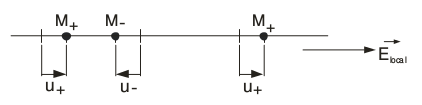
\includegraphics[scale=0.4]{ch3/image1.png}
	\captionof{figure}{ }
	\end{wrapfigure}
Lorsqu'un champ oscillant est présent, les ions vont bouger les uns par rapport aux autres. Considérons le
schéma ci-contre présentant des ions positifs et négatifs et un champ appliqué selon $\vec{1_x}$. En supposant
une force proportionnelle à la déviation de la position du centre d'équilibre des deux voisins, on trouve
\begin{equation}
M_-\dfrac{d^2u_-}{dt^2} = -2C(u_--u_+)-qE_{local}
\end{equation}
où $C$ est le facteur de proportionnalité entre la déviation et la force de rappel et le facteur 2 vient du fait
qu'il y a deux voisins. Pour un ion positif, on trouve 
\begin{equation}
M_+\dfrac{d^2u_+}{dt^2} = -2C(u_+-u_-)+qE_{local}
\end{equation}
Un champ local va exciter chaque type d'ion (local, qui est relié au global, nous y reviendrons). Par combinaison
linéaire, on trouve
\begin{equation}
M\dfrac{d^2u}{dt^2}+2Cu=qE_{local}
\end{equation}
où $u=u_+-u_-$ et où $M= M_+M_-/(M_++M_-)$ est la masse réduite. Par un couple d'ion, le moment dipolaire vaut
$qu$, la polarisabilité est alors donnée par 
\begin{equation}
\alpha(\omega) = \dfrac{q^2}{\epsilon_0(2C-M\omega^2)}
\end{equation}
Ce qui mène à la fréquence de résonance $\omega_{0,a} = \sqrt{\frac{2C}{M}}$. La fréquence de résonance sera
bien plus basse que celle causée par les électrons (en dessous du visible alors que pour ces-derniers c'était
au dessus), tout simplement car $M \gg m_e$.

\subsection{Orientation Polarisation}
Les molécules peuvent avoir des orientations "locales" aléatoire : en l'absence de champ électrique, la 
polarisation macroscopique est nulle. Si on applique $\vec{E}$, ils vont s'orienter dans la même direction
et la polarisabilité serait plus grande. Le processus est cependant assez lent (la molécule doit subir une
rotation) et se détruit facilement (par simple augmentation de la température). La physique statistique nous
donne une valeur que l'on peut associer à ce phénomène
\begin{equation}
\alpha_{as} = \frac{p^2}{3\epsilon_0k_BT}
\end{equation}
Ceci concerne les gaz et les liquides.



\subsection{The Field of Lorentz and the Local Field}
Nous avons précédemment introduit un champ \textit{local}, mais quel mécanisme peut lier ce-dernier au 
champ global? Le champ local peut être différent du global à cause des dipôles. Le champ externe interagit
avec ceux-ci et ils génèrent un second champ qui vient modifier le "champ perçu" par ces mêmes dipôles. Nous
allons ici suivre l'approche de Lorentz et calculer son champ moyen.
\newpage

	\begin{wrapfigure}[5]{r}{3cm}
	%\vspace{-5mm}
	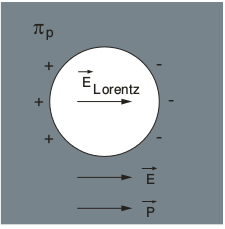
\includegraphics[scale=0.25]{ch3/image2.png}
	\captionof{figure}{ }
	\end{wrapfigure}
Nous allons calculer ce champ moyen en un point en construisant autour de ce point une sphère de rayon 
petit par rapport à l'échelle macroscopique, mais grande par rapport à l'échelle microscopique. A l'intérieur,
on va remplacer la matière continue par pleins de dipôles élémentaires. Le champ local est la somme de trois
contributions
\begin{enumerate}
\item Le champ $\vec{E}$ externe
\item Les dipôles présents
\item Les charges de surface sur la sphère (venant de la construction même de la sphère) : $\sigma_p = -
P\cos\theta$. Lorentz a calculé de que valait ce champ, il a trouvé
\begin{equation}
E_{\text{Lorentz}} = \dfrac{P}{3\epsilon_0}
\end{equation}
Il s'agit donc du champ généré par les charges de surface.
\end{enumerate}
Dans beaucoup de matériaux (si le cercle est centrée sur le point), la contribution des dipôles sera nulle. 
On trouve alors
\begin{equation}
E_{local} = E+\frac{P}{3\epsilon_0}
\end{equation}

\subsection{Clausius-Mosotti Relation}
Utilisons l'expression juste obtenue pour ré-écrire le moment dipolaire
\begin{equation}
p_i = \alpha_i\epsilon_0E_{local} = \alpha_i\epsilon_0\left(E+\dfrac{P}{3\epsilon_0}\right)
\end{equation}
Cette relation relie le force des dipôles au champ local. On peut en déduire le champ de polarisation
\begin{equation}
P = \sum_i N_i p_i = \sum_i N_i\alpha_i\epsilon_0\left(E+\dfrac{P}{3\epsilon_0}\right)
\end{equation}
L'équation est maintenant "fermée". On y voit une sorte de récurrence car le champ local dépend du champ de
polarisation : il faut connaître le 
champ de polarisation pour connaître le champ local puis utiliser ce dernier pour trouver le champ de
polarisation ! Ce qui est beau, c'est que l'on trouve une nouvelle expression pour la susceptibilité électrique
\begin{equation}
\chi_e = \frac{P}{\epsilon_0E}=\dfrac{\sum_i N_i\alpha_i}{1-\frac{1}{3}\sum_i N_i\alpha_i}
\end{equation}
Ce qui est important de comprendre c'est que le champ local défini la polarisabilité et qu'en sommant et 
fermant la relation obtenue on obtient celle-ci. La susceptibilité est donc donnée par la somme des 
polarisabilité divisée par une correction venant du champ local de Lorentz. \\

La loi de Clausius-Mosotti permet de réécrire $E_{local}$ (basée sur l'expression des cristaux cubiques) 
pour obtenir la \textbf{loi de Clausius-Mosotti}
\begin{equation}
\dfrac{\chi_e}{\chi_e+3}=\frac{1}{3}\sum_i N_i\alpha_i
\end{equation}
Avec cette définition de la suceptibilité, la relation de Lorentz devient
\begin{equation}
E_{\text{Local}} = \left(1+\dfrac{\chi_e}{3}\right)E
\end{equation}
L'important est - encore une fois - de voir d'où le problème vient : on travaille sur des effets macroscipique
mais résultant d'un champ local sommé au champ externe.


\subsection{General Dielectric Behaviour}
Reprenons les précédents résultats. La polarisation électronique se situe dans l'UV (une ou plusieurs 
résonances). La polarisation se situe (une ou plusieurs résonances)  dans l’infrarouge et la polarisation 
d'orientation à une fréquence critique dans les radio.
\begin{center}
	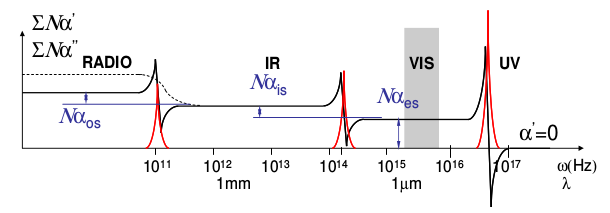
\includegraphics[scale=0.6]{ch3/image3.png}
	\captionof{figure}{Attention, les résonances montent d'abord puis elle descendent, pas l'inverse!}
\end{center}
On voit que les différentes résonances ne sont pas dans le visible. Cependant, le nombre de résonances "avant
et après" le visible influence la valeur "du visible" : les résonances ont une contribution indirectes. Pour
récapituler, $\alpha$ est la tendance à polariser une charge \textbf{unique} (ion, électron,\dots) alors que
$\chi$ est la tendance à polariser \textbf{tout} le matériau. La loi de Clausius-Mozotti donne la relation entre
$\alpha$ et $\chi$.


\section{Microscopic Theory for Conductors and Semiconductors}
Dans les dielectriques, la réaction de $E$ est décrite par $P$. Dans un conducteurs, par le courant $J$ car
les électrons sont libres de se mouvoir\footnote{"\textit{Le modèle de Drude est \textbf{vraiment à connaître}}".}.

\subsection{The 1D Drude Free-Electron Model for Metals}
Soit des ions à positions fixes et des électrons dans la bande de conduction : pas d'interactions entre les deux
espèces, mais les électrons accélèrent en présence de $\vec{E}$. Parfois, les $e^-$ collisionnent avec les ions
ou les impuretés. La probabilité de collision sur $dt$ est donnée par $dt/\tau$. Les collisions ne sont pas
élastiques, mais la vitesse après collision est dictée par la condition d'équilibre thermique. Sans $\vec{E}$, 
la vitesse moyenne des $e^-$ et donc $J$ est nul.\\

Soit $E(t)$ et un ensemble d'$e^-$ avec une position moyenne $x$. Négligeons la variation spatiale. L'impulsion
linéaire moyen $m\text{d}x/\text{d}t$ au temps $t+\text{d}t$ (où $dt\ll \tau$) est composé de deux contributions
\begin{enumerate}
\item La fraction des électrons qui voient leurs impulsions augmentées sous l'influence de la force $-eE$
\begin{equation}
\left(1-\dfrac{\text{d}t}{\tau}\right)
\end{equation}
\item La fraction $\text{d}t/\tau$ des électrons qui n'obtiennent pas d'impulsion à cause de la collision avec
un ion.
\end{enumerate}
L'impulsion moyenne en $t+\text{d}t$ devient alors
\begin{equation}
m\dfrac{\text{d}x}{\text{d}t}(t+\text{d}t) = \left(1-\dfrac{\text{d}t}{\tau}\right)\left(m\dfrac{\text{d}x}{
\text{d}t}(t)-eE(t)\text{d}t)\right)
\end{equation}
Ceci mène à l'équation de mouvement
\begin{equation}
m\dfrac{\text{d}^2x}{\text{d}t^2}=-\dfrac{m}{\tau}\dfrac{\text{d}x}{\text{d}t}-eE
\end{equation}
où l'on reconnaît un terme de \textit{damping} à droite. Notons qu'il y a \textbf{également} des électrons
liés dans un conducteurs, dans les basses couches. Sachant que $J = -Ne\dfrac{\text{d}x}{\text{d}t}$
\begin{equation}
\dfrac{\text{d}J}{\text{d}t} = -\dfrac{J}{\tau}+\dfrac{Ne^2}{m}E
\end{equation}
Ce qui devient, en régime harmonique $e^{i\omega t}$
\begin{equation}
J(\omega) = \dfrac{Ne^2\tau}{m(1+i\omega\tau)}E(\omega)
\end{equation}
Connaissant la loi d'Ohm
\begin{equation}
\sigma(\omega) = \dfrac{Ne^2\tau}{m(1+i\omega\tau)}
\end{equation}
Il s'agit de la \textbf{complex frequency dependant conductivity}. \\

Nous avions trouvé au chapitre 2
\begin{equation}
\epsilon = \epsilon_0\left(1+\chi-i\dfrac{\sigma}{\omega\epsilon_0}\right) = \epsilon_0\left(1+\chi+
\dfrac{Ne^2}{m\epsilon_0}\dfrac{1}{-\omega^2+i\omega/\tau}\right)
\end{equation}
Ceci est facile à interpréter si l'on 
remarque que $1/\tau$ est la fréquence de collision. A basse fréquence, la partie complexe de la constante
diélectrique deviant importante (par les relations de KK, cela va avoir une influence sur la partie réelle). Si en plus plus $\omega \gg 1/\tau$, le terme d'amortissement peut être
négligé et la courant d'électron libre contribue négativement à la constante diélectrique. La susceptibilité
équivalente due à la conduction ("plasma" idéal) est 
\begin{equation}
\chi_{\text{conduction}} = -\dfrac{\omega_p^2}{\omega^2}
\end{equation}
Qui devient $-1$ à la fréquence plasma $\omega_p = \sqrt{(Ne^2	)/(m\epsilon_0)}$.




\subsection{Cubic Crystals}
Le reste du chapitre n'est pas pour l'examen.
































\chapter{Numerical methods for boundary value problems}
As seen, one concern for boundary value problems is the CPU time and the memory requirements. Most of the problems in fluid mechanics are non-linear and one way to solve them is to use Newton's method, consisting in solving a system of linear equations. We will discuss about the accuracy, stability and convergence of iterative solution processes. 

\section{Direct methods for the solution of linear systems (Gaussian elimination \& variants)}
These are not discussed here but they are all based on Gaussian elimination, LU factorization. We will just recall that for a sparse matrix in 1D the CPU cost is of order $\mathcal{O}(nb^2)$ and the memory $\mathcal{O}(nb)$ where $n$ is the number of unknowns and $b$ the bandwidth. In 2D: $N=nm$, $b=m$, this becomes excessively costly. Because of this cost the direct method have been excluded from numerical computation for long time ago. In mechanics the direct methods are used, we can solve with much less dense grids for compared to fluid dynamics. This is why in CFD one has tried to look for alternative approaches. 

\section{Iterative methods}
\subsection{Fixed point methods}
If we want to solve $Ax=b$, the idea is to replace this by solving a sequence of linear problems, iterates $x^k$ of the type: 

\begin{equation}
Bx^{(k+1)} = b + (B-A)x^{(k)}
\end{equation}

There is two conditions for this to be competitive, the cost of every step has to be low, much smaller than the direct method. The second condition is that the method converges fast so that the global cost does not exceed direct method.\\

The first condition is satisfied if the matrix $B$ is (a product of) diagonal or (upper or lower) triangular matrices, diagonal cost is $\mathcal{O}(n)$ and the other $\mathcal{O}(nb)$. For the second condition, let's multiply by $B^{-1}$:

\begin{equation}
x^{(k+1)} = B^{-1}b + (I - B^{-1}A) x^{(k)}\qquad 
\tilde{x} = B^{-1}b + (I - B^{-1}A) \tilde{x}
\end{equation}

where $\tilde{x}$ is the converged solution $A\tilde{x}=b$. If we make the difference we will get: 

\begin{equation}
x^{(k+1)}-\tilde{x} = e^{k+1} = (I - B^{-1}A)[x^{(k)}-\tilde{x}] = Ge^{(k)}
\end{equation}

Where we make appear the error on the solution. To have the fastest convergence, the coefficients of $G$ should be as small as possible. The simplest choices for B are the followings: $B=I$ (Richardson) or $B=A_{D}$ (diagonal part of A) (Jacobi). 

\begin{itemize}
\item[•] $B=I$: this is the simplest one, Richardson's method: 

\begin{equation}
x^{(k+1)} =  x^{(k)} + (b-Ax^{(k)}) \qquad \Rightarrow x^{(k+1)}_i =  x^{(k)}_i + (b_i-\sum _{j=1}^n a_{ij} x_j^{(k)})
\end{equation}

\item[•] The jacobi method would consist in ($A_L,A_U$ are the lower and upper triangular matrices): 

\begin{equation}
Bx^{(k+1)} =  b + (B-A)x^{(k)} = b - (A_L+A_U)x^{(k)}  \qquad \Rightarrow a_{ii} x_i^{(k+1)} = b_i - \sum _{j=1,j\neq i}a_{ij}x_j^{(k)}
\end{equation}

\item[•] $B = A_L + A_D$ or $B = A_D + A_U$, we can take a combination of triangular parts and diagonal part, as suggested by the Gauss-Seidel mthod.

\begin{equation}
\begin{aligned}
&(A_L + A_D)x^{(k+1)} = b - A_U x^{(k)} \qquad \sum_{j=1}^i a_{ij}x_j^{(k+1)} = b_i - \sum _{j=i+1}^n a_{ij}x_j^{(k)}\\
&(A_D + A_U)x^{(k+1)} = b - A_L x^{(k)} \qquad \sum_{j=i}^n a_{ij}x_j^{(k+1)} = b_i - \sum _{j=1}^{i-1} a_{ij}x_j^{(k)} 
\end{aligned}
\end{equation}

\item[•] These two algorithms being asymetric, it is preferred to combine first a substep of the first then a substep of the second si that we get the Symmetric Gauss-Seidel (SGS): 

\begin{equation}
(A_L + A_D)x^* = b - A_U x^{(k)} \qquad (A_D + A_U)x^{(k+1)} = b - A_L x^* = A_D x^* + A_U x^{(k)}
\end{equation}

It can be easily shown that the last expression can be compacted by defining:

\begin{equation}
B_{SGS} = (A_L + A_D) A_D^{-1}(A_D + A_U)\qquad \Rightarrow
(A_L + A_D) A^{-1}_D (A_L+A_U)\delta _x = b_i - Ax^{(k)} 
\end{equation}

%So that we get a system
%\begin{equation}
%(A_L + A_D) \delta _x ^* = b-Ax^{(k)}
%(A_L + A_U) \delta _x  = A_D \delta _x^*
%\end{equation}

\item[•] We can go further and use an additional parameter $\omega$ to control the convergence (relaxation parameter), the optimum omega is an over relaxation >1: 

\begin{equation}
B = A_L + \frac{A _D}{\omega}
\end{equation}

when applied to Gauss-Seidel normal. We can also apply to symmetric one $\rightarrow$ symmetric successive over-relaxation SSOR. When you write the system in the iterative way, we remark that it is in fact a richardson method for the system $B^{-1}Ax= B^{-1}b$, indeed if we do Richardson on that . Everything is based on the richardson and this is why we call $B^{-1}Ax = B^{-1}b$ preconditioning system. 

\subsection{Convergence of the fixed point method}

When expressing the second condition, we found: 

\begin{equation}
x^{(k+1)}-\tilde{x} = e^{(k+1)} = [I-B^{-1}A]e^{(k)} = Ge^{(k)}
\end{equation}

The convergence condition is $|\rho (G)|\leq 1$ for the amplification matrix at each iteration. Assuming that has a complete set of eigenvalues and lin. ind. eigenvectors: 
\begin{equation}
e^{(0)} = a_i V_i \qquad e^{(1)} = Ga_i V_i  = a_i GV_i = a_i \lambda ^{(1)}V_i \qquad e^{(k)}=G^k a_iV_i = \lambda ^{(i)^k}a_iV_i
\end{equation}

STOPPED HERE

The condition can be reexpressed by considering the spectral radius of G (largest modulus eigenvalue) respects $\rho _G = |\lambda (G)|_{max}<1$. Asymptotically $e^{k+1} = |\lambda|_{max}e^k$. The convergence speed $\frac{1}{n_{it}}$ needed to reduce the error by 1 order of magnitude. It is always the bigger eigenvalues are dominating: 

\begin{equation}
e^{k+n} = |\lambda _{max}|^n e^k \qquad \frac{e^k}{e^{k+n}} = \frac{1}{|\lambda _{max}|^n} \Rightarrow 1 = -n\log |\lambda _{max}| \qquad \frac{1}{n} = V_C = -\log |\lambda _{max}| = - \log \rho
\end{equation}

It is shown in the syllabus (he skip details) that A resulting from the discretization of Laplace's equation on a grid with $\Delta x= \Delta y = h$: 

\begin{equation}
\rho _{G,J} = 1-\mathcal{O}(h^2) \Rightarrow V_c = \mathcal{h^2} \qquad \rho _{G,S} = \rho _{G,J}^2 \Rightarrow V_{C,GS} = 2V_{C,J}
\end{equation}

SOR : $\exists$ an optimum $\omega \rightarrow $ at the optimum $\omega, V_C = \mathcal{O}(h)$. 
\end{itemize}
\section{Better iterative schemes ? }
Consider: 

\begin{equation}
B^{-1}A x = B^{-1}b \qquad A' = b'
\end{equation} 

We have that in iteration mode: 

\begin{equation}
x^{(k+1)} = b' + (I-A')x^{(k)} = x^{(k)} + \underbrace{b' - A' x^{(k)}}_{r^{(k)}}
\end{equation}

Then the residual $r^{(k)}$: 

\begin{equation}
x^{(k+1)} = x^{(k)} + r^{(k)} = x^{(k-1)} + r^{(k-1) } + r^{(k) } = x^{(0)} + r^{(0) } + r^{(1) } + \dots + r^{(k) }
\end{equation}

The residual is defined such that: 

\begin{equation}
r^{(k+1)} = b' - A' x^{(k+1)} = b' - A' [x^{(k)}+r^{(k)}] = r^{(k)} - A' r^{(k)} = (I-A')r^{(k)} 
\end{equation}

So that we can write: 

\begin{equation}
x^{(0)} + [I + (I-A)+ (I-A)^2+ \dots + (I-A)^k] r^{(k)}
\end{equation}

We see that we have a polynomial of $A$, with $V$ belonging to $K_k (A,r_0) = span (r_0,Ar_0,A^2r_0 ... A^k r_0)$, we search for a better space. 

\subsection{Kvylov subspace methods}
Is it possible to construct a better iterate in the same vector space ? 2 strategies: 1) find the iterate such that $r^{(k+1)}$ is perpendicular to the vector space $K_k(r_0,A)$ . 2) find the iterate that minimizes the $||r^{k+1}|| \Leftrightarrow r^{(k+1)}\perp AK_k (r_0,A)$ so that $||b-Ax^{(k+1)}||_{min}$. Let's apply to 

\begin{equation}
\begin{aligned}
&x^{(0)} \quad r^{(0)} = b-Ax^{(0)} \\
&x^{(1)} = x^{(0)} + \alpha r^{(0)}
\end{aligned}
\end{equation}

The first method gives: 

\begin{equation}
\begin{aligned}
&r^{(1)} = b-Ax^{(1)} = r^{(0)} - \alpha A r^{(0)}\\
&r^{(1)} \perp r^{(0)} \quad (r^{(0)}- \alpha A r^{(0)}, r^{(0)}) = 0 \\
&r^{(0)}, r^{(0)} - \alpha (Ar^{(0)}, r^{(0)}) = 0\\
&\alpha = \frac{r^{(0)},r^{(0)}}{r^{(0)},Ar^{(0)}} 
\end{aligned}
\end{equation}

The second method gives: 

\begin{equation}
\begin{aligned}
&||r^{(1)}||^2 = r^{(0)}-\alpha A r^{(0)}, r^{(0)}-\alpha A r^{(0)} = (r^{(0)},r^{(0)}) - 2\alpha (r^{(0)},A r^{(0)})+ \alpha ^2(Ar^{(0)}, Ar^{(0)})\\
&\Rightarrow \frac{d}{d\alpha} ||r^{(1)}||^2 = -2(r^{(0)}, Ar^{(0)}) + 2\alpha (r^{(0)}, A r^{(0)})
\end{aligned}
\end{equation}

Num
\begin{equation}
^\alpha _{opt} = \frac{r^{(0)},Ar^{(0)}}{Ar^{(0)},Ar^{(0)}} \Leftrightarrow (r_{opt}^{(1)}= r^{(0)}-\alpha _{opt} A r^{(0)}, Ar^{(0)}) = 0
\end{equation}

page 126 syllabus. DONT DO THE CONVERGENCE 


\section{Stability of the space discretization}
We want to look to the stability of the space discretization, we are dealing with boundary conditions and assume that we have a strategy to solve the problem, what about the stability of the resulting solution ?

\subsection{Stability for advection-dominated problems}
We have full advection problems :
\begin{equation}
\frac{\D F_i}{\D x_i} = 0
\end{equation}

We have advection diffusion problems: 

\begin{equation}
a _i \frac{\D u}{\D x_i} = \alpha \frac{\D ^2 u}{\D x_j \D x_j}
\end{equation}

And the advection reaction problems

\begin{equation}
a_i \frac{\D u}{\D x_i} = S_i
\end{equation}

We take as model equation the advection-diffusion in 1D: 

\begin{equation}
a \frac{du}{dx} = \alpha \frac{d^2}{dx^2}
\end{equation}

and we assume that $u(0)= u_{in}$ and that $u(1) = u_{out}$ in a range $0,1$. The solution will be in the form $e^{rx}$ so that $ar = \alpha r^2\Rightarrow r = 0, r = a/\alpha$. We have thus that $u = c_1 + c_2 e^{ax/\alpha}$ where we find the constants with the boundary conditions: 

\begin{equation}
u_{in} = c_1 + c_2 \qquad u_{out} = c_1 + c_2e^{aL/\alpha}
\end{equation} 

where $aL/\alpha$ is the Pecklet number (Reynolds in thermo). The constants are: 
\begin{equation}
\begin{aligned}
&c_2(e^{P_e}-1) = u_{out} - u_{in} \qquad c_1(e^{P_e}-1) = u_{in}e^{Pe} - u_{out} \\ 
&u = \frac{u_{in}e^{Pe}-u_{out}}{e^{Pe}-1}+ \frac{u_{out}-u_{in}}{e^{Pe}-1}e^{\alpha x	\alpha} = u_{in} + (u_{out}-u_{in} \frac{e^{\frac{ax}{\alpha}}-1}{e^{Pe}-1})
\end{aligned}
\end{equation}

The central discretization is 
\begin{equation}
\Delta w = h \quad a\frac{u_{i+1}-u_{i-1}}{2h} = \alpha \frac{u_{i+1}-2u_i+u_{i-1}}{h^2}
\end{equation}

Knowing that $u_{i+1}= gu_i, u_i = g^i$ such that 

\begin{equation}
\begin{aligned}
&\frac{h^2}{\alpha} \times a\frac{g^2-1}{2h} = \alpha \frac{g^2 - 2 g +1}{h^2}\\
&\frac{ah}{\alpha} (g^2-1) = g^2 -2g +1 \Rightarrow g^2 (1- \frac{Pe}{2})-2g + 1 + \frac{Pe}{2} = 0\\
&(g-1)\underbrace{(g(1-\frac{Pe}{2})-(1+\frac{Pe}{2}))}_{g = \frac{1+Pe/2}{1-Pe/2}}
\end{aligned}
\end{equation}

The boundary conditions applied to find the constants: 
\begin{equation}
u_i = C_1 A^i + c_2 \left(\frac{1+Pe/2}{1-Pe/2} \right) = u_{in} + (u_{out}-u_{in})\frac{g^1 -1 }{g^n -1}
\end{equation}

figure 130 we observe that the exact solution is monotonically increasing while the numerical solution shows oscillations. It is easy to observe where the oscillations comes from. When the Pe > 2, the g is negative and thus the solution will change sign at every computation. So what to do ? Let's refine the mesh to reduce h. However in several simension we can have coexistence of regions of strong gradient $\alpha / a$. How do we stabilize the solution ? 

\subsubsection{Stabilization of the solution}
By using an upwind scheme using the advection term. We go from central advection to central advection: 

\begin{equation}
\begin{aligned}
&a \frac{u_i - u_{i-1}}{h} = \alpha \frac{u_{i+1}-2u_i + u_{i-1}}{h^2} \Rightarrow Pe  (u_i - u_{i-1}) = u_{i+1}-2u_i - 2u_i + u_{i-1}\\
&0 = g^2 - (2 + Pe) u_i +(1+Pe) u_i + 1\\
&(g-1)(g-(1+Pe)) \Rightarrow 2 + V_e \ roots \rightarrow Non oscillation
\end{aligned}
\end{equation}

We can see that :

\begin{equation}
\frac{u_i - u_{i-1}}{h} = \frac{u_{i+1}-u_{i-1}}{2h} - \frac{u_{i+1}-2u_i +u_{i-1}}{2h} \qquad \Rightarrow a \frac{u_{i+1}-u_{i-1}}{2h} = \frac{u_{i+1}-2u_i+  u_{i-1}}{h^2}(\alpha + \zeta \frac{ah}{2})
\end{equation}
We have an artificial diffusion term. 
read 131. 

\subsubsection{Galerkin FE discretization}
\begin{equation}
a\frac{du}{dx}= \alpha \frac{d^2u}{dx^2} \qquad a\frac{du}{dx} - \alpha \frac{d^2u}{dx^2} = 0 \qquad \int _0^L (\phi _i \frac{du^h}{dx}+ \alpha \frac{d\phi _i}{dx}\frac{du^h}{dx})\, dx - \cancel{[\phi q]_0^L }
\end{equation}

The last term goes away with dirichlet condition. We have $\phi$ with contribution of element A and element B: 

\begin{equation}
A: [\frac{a}{2}\frac{u_i - u_{i-1}}{h}+\alpha \frac{1}{h} \frac{u_i - u_{i-1}}{h}]h
B: [\frac{a}{2}\frac{u_{i+1} - u_{i}}{h}-\alpha \frac{1}{h} \frac{u_{i+1} - u_{i}}{h}]h
\end{equation}

The sum of the two gives something central so we have the same stabilization problem

\begin{equation}
\left(\frac{u_{i+1}-u_{i-1}}{2h}-\alpha \frac{u_{i+1}-2u_i+u_{i-1}}{h^2} \right)h = 0
\end{equation}

If we do the least square: 

\begin{equation}
\int \underbrace{\frac{\D r^*}{\D u_i}}_{\left( a\frac{d\phi _i}{dx} - \cancel{\frac{d^2\phi _i}{dx^2}} \right)}\times \left( a\frac{du^h}{dx}-\cancel{\alpha \frac{d^2uh}{dx^2} }\right) \, dx
\end{equation}

Cancelation applies for piecewise linear elements. We will have an extra term 

\begin{equation}
\int _0 ^L \tau a^2 \frac{d\phi _i}{dx}\frac{du^h}{dx}dx
\hat{\alpha} = \tau a^2 = \zeta \frac{ah}{2} \Rightarrow \tau = \zeta \frac{h}{2a}
\end{equation}

4.47 there is one alpha too much. Some illustrations. 

\subsection{Pressure stabilization for incompressible flows}
Which problem ? Take the Stokes equation: 

\begin{equation}
\nabla u = 0 \Rightarrow \cancel{(\bar{u} \nabla)} \bar{u}= - \nabla P + \nu \nabla ^2 \bar{u}
\end{equation}

Consider a cartesion mesh of spacing $\Delta x = \Delta y = h$ so that the central discretization gives: 

\begin{equation}
\begin{aligned}
&\frac{u_{i+1,j}-u_{i-1,j}}{2h}+ \frac{v_{i,j + 1}-v_{i,j-1}}{2h} = 0 \\
&0 = - \frac{P_{i+1,j} - P_{i-1,j}}{2h}+ \frac{\nu}{h^2}(\delta _x^2+ \delta _y^2)u_{ij}\\
&0 = - \frac{P_{i,j+1} - P_{i,j-1}}{2h}+ \frac{\nu}{h^2}(\delta _x^2+ \delta _y^2)v_{ij}
\end{aligned}
\end{equation}

Let's look to diffusive terms: 
\begin{equation}
\begin{aligned}
&0 = -\left( \frac{P_{i+2,j} - P_{i,j}}{2h} - \frac{P_{i,j} - P_{i-2,j}}{2h} \right) \frac{1}{2h} + \frac{\nu}{h^2}(\delta _x^2+ \delta _y^2)\left( \frac{u_{i+1,j}- u_{i-1,j}}{2h} + \frac{v_{i,j+1}- v_{i,j-1}}{2h} \right) \\
&-\left( \frac{P_{i+2,j} - P_{i,j}}{2h}- \frac{P_{i,j} - P_{i-2,j}}{2h} \right) \frac{1}{2h} 
\end{aligned}
\end{equation}

In fluid mechanics, we always need a central scheme and a bit of stabilization. It is not as structural stability where we are happy with the Galerkin method. 

\chapter{Compression systems}
\section{Introduction and different types of compressors}
\subsection{Purpose and compressor types}
Turbocompressors are systems used to convert shaft mechanical energy into fluid pressure and kinetic energy. The fluid can be air and other special gases like nitrogen or whatever. When the inlet pressure is lower than atmospheric one and that output pressure is the atmospheric pressure we speak of \textbf{vacuum pump} and when the exhaust pressure is low with one stage of blades it is a \textbf{fan} or a \textbf{ventilator}.

\subsubsection{Reciprocating / piston compressors}
\wrapfig{9}{l}{3}{0.2}{ch5/1}
There exists two big families of compressors: the volumetric compressors and the turbocompressors. The first family consists in machines that compress by decreasing the gas volume (reciprocating compressors for ex) and the second compresses through a rotor that redirects the flow. A problem of the volumetric compressors is the lack of continuity due to the injection, we need a tank. We also need lubricant where metal-metal contact happens. Leakage around the piston is also a problem and the friction increases the need for maintenance. 
Discharge pressures can go from very low pressures to very high (180 MPa)

\subsubsection{Rotary vane compressors}
\wrapfig{8}{r}{3}{0.3}{ch5/2}
Rotary compressors are composed of a rotor with blades inserted in radial slots, placed offset in a larger circular (or complex shape) housing. When the machine rotates, the blades are moving in the slots so that the volume which confine the air decreases with the angle. This is similar to the piston compressor but is quiter and can go up to 1.3 MPa in one stage. Its efficiency is around 90\% .

\subsubsection{Roots compressors and rotary screw compressors} 
\minifig{ch5/3}{ch5/4}{0.3}{0.3}{0.4}{0.4}

Roots compressors pressure ratio and mass flow rate are very low but works very smoothly (low vibrations and noise), \autoref{ch5/3}. Rotary screw compressors are composed of two meshed rotating positive-displacement helical screws in order to force the fluid in smaller spaces. These are used for continuous operation, has a power between 2.2 up to 890 kW and pressures up to 8.3 MPa. Types: oil flooded, water flooded and dry. The longer the screw the higher the compression ratio. 

\subsubsection{Turbocompressors}
\wrapfig{8}{l}{6}{0.3}{ch5/5}
They are similar to the pumps, centrifugal compressor composed of a bladed rotor that gives kinetic energy to the fluid and then it is converted into pressure in the divergent duct. They can have very high exhaust pressures (up to 69 MPa with multistage). Almost no metal-metal contact so the maintenance request is very low. 

\ \\
For high flow rate and compact design we use the axial flow compressors (\autoref{ch5/5}). They are almost always composed of multistage, the cross sectional area decreases at each stage, one rotor followed by one stator. 

\subsection{Use of different compressor types}
They differs from diverse parameters: 

\begin{itemize}
\item[•] Mass flow rate: huge for axial turbocompressors, large for centrifugal turbo and rather small for all other \\
\item[•] Maximum ratio per stage: large for centrifugal turbo, medium for piston compressors and very small for axial turbo, but axial turbo is the only one where it is easy to put series of stages and reach very high ratios
\item[•] Poor air (no pollutants): axial and centrifugal turbo are very good for that, piston and rotary vane types are very poor because of the lubricant. 
\end{itemize}

\section{Fundamental equations for gas compression systems}
\subsection{Definitions and nomenclature}
\subsubsection{Admission and exhaust pressure}
The volume from which we take air is called \textbf{aspiration medium} or \textbf{aspiration environment} and the pressure there $p_0$ is the \textbf{aspiration pressure}. Similarly for the exit we have the \textbf{exhaust} medium, environment and pressure $p_1$. The losses in the piping are not negligible. 

\subsubsection{Compressor pressure ratio}
It is defined in terms of the \textbf{total} pressure, because in the theorem of kinetic energy the velocity intervenes: 

\begin{equation}
\pi _c = \frac{p_{t, out}}{p_{t, in}}
\end{equation}

\subsubsection{Flow rate}
Mass flow rate (kg/s) are used instead of volumetric flow rate ($m^3$/s) because if we use the second we have to specify the conditions at the exhaust and the intrance (change in density), while mass flow rate stays constant (very small leak losses).

\subsubsection{Specific energy consumption}
The specific consumption is the ratio between the driving power and the volumetric flow rate: 

\begin{equation}
SFC = \frac{P_m}{Q_{out}}
\end{equation} 

This is for the manufacturer not for us. For large to medium, water cooled compressors it is about 280-310 J/l and can be 3-5\% higher for air cooled (1\% absorbed by cooling fan). 

\subsection{Fundamental thermodynamics law}
\subsubsection{Introduction}
We will only consider steady state, so not the transients (accelerations and decelarations of the machine) and variations of aspiration and exhaust conditions. 

\minifig{ch5/6}{ch5/7}{0.4}{0.4}{0.4}{0.4}

We will apply the first principle and second principle of thermodynamics and also the kinetic energy equation on a given mass of gas contained initially between the volume $A_0, A_1$ and a period later so at $t+\Delta t$ between $A_0', A_1'$ as represented on the figures for the reciprocating and turbo compressors. For the piston, the time interval corresponds to a piston period while for turbocompressors it is arbitrary. The mass of air between $A_0$ and $A_0'$ is always the same as the one contained in $A_1$ and $A_1'$, the mass between $A_0'$ and $A_1$ is also always constant and thermodynamic variables are all the same at $t$ and $t+ \Delta t$.

\subsubsection{Use of the energy equation}
He skipped all the equations before. The energy equation is: 

\begin{equation}
q + p_0 \nu_0 - p_1 \nu _1 + w_i = u_1 - u_0 + \frac{v_1 ^2 - v_0^2}{2} + g(z_1-z_0)
\end{equation}

Combining pressure and $u$ terms to get $h$ and neglecting the level difference $\Delta z$: 

\begin{equation}
q + w_i = h_1 - h_0  \qquad \Rightarrow (q= 0) \ w_i = \Delta h = c_p \Delta T\qquad  \Leftrightarrow P_i = \dot{m} c_p \Delta T
\end{equation}

\subsubsection{Second fundamental thermodynamics law}
We have that: 

\begin{equation}
ds = \delta q/T + ds_{irr} \quad \Rightarrow Tds = dh - \nu dp = \delta q + ds_{irr} \quad \Rightarrow h_1 - h_0 - \int _0 ^1 \nu dp = q + \int _0 ^1 Tds_{irr}
\end{equation}

We see that the integration gives something similar to what we had before but with an additional irreversible term. 

\subsubsection{Kinetic energy equation}
By combining the two last equations we got: 

\begin{equation}
w_i = \int _0 ^1 \nu dp + \int _0 ^1 Tds_{irr}
\end{equation}

We see that the work provided by the piston or the rotor is used to increase the pressure and to compensate the losses due to irreversibility. 

\subsubsection{Total system of equations}
\theor{
Total energy equation: 
\begin{equation}
q + w_i = h_1 -h_2 
\end{equation}

Kinetic energy equation: 

\begin{equation}
w_i = \int _0 ^1 \nu dp + \int _0 ^1 Tds_{irr}
\end{equation}

Global thermodynamic equation

\begin{equation}
\int _0^1 Tds = h_1 - h_0 - \int _0 ^1 \nu dp = q + \int _0 ^1 Tds_{irr}
\end{equation}
}\ \\

\section{Compression of perfect gases}
\subsection{Reference compression modes}
Since it is impossible to model the real compression mode because of the irreversibilities. We will study 3 types of compression to see the effects of some parameters: 

\begin{itemize}
\item[•] Reversible isothermal compression 
\item[•] Reversible adiabatic compression (isentropic compression)
\item[•] Polytropic compression
\end{itemize}

The fluid is considered to be a perfect gas with $c_p = cst$.

\subsection{Reversible internal compression}
\subsubsection{Internal work and internal power}
Assuming the compressor to be highly cooled, we can assume isothermal process. We neglect irreversibilities and thus the energy equation of previous section becomes: 

\begin{equation}
w_{it} + q = h_1 -h_0 = c_p\Delta T = 0 \qquad w_{it} = -q
\end{equation}

The internal work is thus equal to the heat to be extracted from the compressed gas to keep the temperature constant. The kinetic energy equation gives: 

\begin{equation}
w_{it} = \int _0 ^1 \nu dp = RT_0 \ln \pi _c \qquad \Rightarrow P_{it} = \dot{m} rT_0 \ln \pi _c
\end{equation}

where we used the perfect gas relation $\nu = rT_0/p$. We deduce that indeed higher pressure ratios require higher works, but also higher temperatures require higher work (not the same in winter and summer). 

\subsubsection{Presentation on the entropy diagram}
\wrapfig{8}{l}{4.5}{0.3}{ch5/8}
Since the inlet conditions $p_0,T_0$ are known, we have the aspiration point on the T-S diagram. To obtain the exhaust conditions it is sufficient to keep the temperature constant and to jump on $p_1$ curve (reversible so straight line).  From the fundamental second law: 

\begin{equation}
q = \int _0 ^1 Tds = T_0 (s_{1t}- s_0) = \overline{0 - 1_t}
\end{equation}

We see that the heat extracted corresponds to the area corresponding to the projection of the $\overline{0-1_t}$ curve on s axis. Covered anticlockwise it is the negative direction so we have the heat and clockwise direction corresponds to $w_i$: 

\begin{equation}
w_i = \overline{1_t - 0}
\end{equation} 

\subsection{Isentropic compression}
This time we consider adiabatic and reversible compression $q=0 = \int Tds_{irr}$. The energy equation gives: 

\begin{equation}
w_{is} = h_1 - h_0 = c_p T_0 \left(\frac{T_{1s}}{T_0} - 1\right) = c_p T_0 \left(\pi ^{\frac{\chi - 1}{\chi}} _c- 1\right)
\end{equation}

where the compression ratio comes from isentropic law. On the other hand: 

\begin{equation}
r = c_p - c_v = c_p \left( 1 - \frac{1}{\chi} \right) \qquad \Rightarrow c_p = \frac{\chi}{\chi -1} r
\end{equation}

Injecting this in previous expression: 

\begin{equation}
w_{is} = \frac{\chi}{\chi -1} r T_0 \left(\pi ^{\frac{\chi - 1}{\chi}} _c- 1\right)
\end{equation}

Again work is increasing with compression ratio and it is shown with an example in the syllabus that it is higher than the iso-T case! 

\subsubsection{Presentation on the entropy diagram}
\wrapfig{8}{r}{4.5}{0.3}{ch5/9}
Consider an additional point which is $1_t$ for this diagram, the point $1_s$ is obtained with the isentropic evolution. Since temperatures are the same at $1_t$ and $0$, $h_{1s} - h_0 = h_{1s} - h_{1t}$. If we imagine an evolution between $1_t and 1_s$ and apply the second fundamental relation: 

\begin{equation}
\int _{1t} ^{1s} = h_{1s} - h_{1t} + \cancel{\int \nu dp} = w_{is} = \overline{1_t - 1_s}
\end{equation}

That projection area is larger than the iso-T case as deduced. 

\subsection{Polytropic compression}
\subsubsection{Definition}
The evolution that matches the best the real life evolution is the polytropic evolution. The final point ($p_1,T_1$) is the same as the real life while not in iso-T and iso-S. The evolution respects: 

\begin{equation}
p_1\nu_1^" = p_2\nu _2^"
\end{equation}

This injected in the perfect gas law: 

\begin{equation}
\frac{T_1}{T_0} = \left( \frac{p_1}{p_0}\right)^{\frac{n-1}{n}} \qquad T_1\nu_1^{n-1} = T_0\nu_0^{n-1}
\end{equation}

where $n$ is the polytopric exponent, similar to the $\gamma$ of the isentropic evolution. 

\subsubsection{Experimental determination of the polytropic exponent}
It is easily found as follows: 

\begin{equation}
\frac{T_1}{T_0} = \left( \frac{p_1}{p_0}\right)^{\frac{n-1}{n}} \Leftrightarrow \frac{n}{n-1} = \frac{\ln \frac{T_1}{T_0}}{\ln \frac{p_1}{p_0}} \qquad \Rightarrow n = \frac{\ln \frac{p_1}{p_0}}{\ln \frac{p_1}{p_0} - \ln \frac{T_1}{T_0}}
\end{equation}

\subsubsection{Internal work and internal power}
Again, we can neglet irreversibility, and using the kinetic energy equation we can get (no development given): 

\begin{equation}
w_{ip} = \frac{n}{n-1}rT_0\left( \pi _c ^{\frac{n-1}{n}} -1 \right)
\end{equation}

\subsubsection{Presentation on the entropy diagram}
A distinction has to be made between cooked systems and adiabatic systems

\wrapfig{6}{l}{4.5}{0.3}{ch5/10}
\paragraph{Cooled compression}
In practice, the cooling is larger than the irreversible effect so that the thermodynamic relation tells that entropy decreases: 

\begin{equation}
\int _0^1 Tds = q + \int Tds _{irr} \qquad \Leftrightarrow \overline{1-0} = -q
\end{equation}

We see that the projection area under the curve 1-0 (positive direction) corresponds to the heat to be extracted. On the other hand, the energy equation tells that: 

\begin{equation}
w_i + q = h_1 - h_0 = h_1 - h_{1t} = \overline{1_t - 1} \qquad \Leftrightarrow w_{ip} = \overline{1_t -1 -0}
\end{equation}

\wrapfig{6}{l}{4.5}{0.3}{ch5/11}
\paragraph{Adiabatic compression}
A real compression is non-reversible and adiabatic. The polytropic compression that we use is reversible but not adiabatic anymore. Indeed, the real point on the graph would be not reachable in that case since reversible + adiabatic = isentropic. In fact, the effects of the non reversibilities are replace by an addition of heat: 

\begin{equation}
w_i + q = h_1 - h_0 = h_1 - h_{1t} = \overline{1_t - 1} \qquad \int _0^1 Tds = q = \overline{0-1}
\end{equation}

Substraction of the two projection surfaces gives: 

\begin{equation}
w_{ip} = \overline{1_t - 1 - 0}
\end{equation}

\subsection{Cooled compressors - refrigerated compression}
\subsubsection{Application and presentation on the entropy diagram}
Piston compressors are cooled because the lubricant looses its properties at very high temperature and then can pollute the air. \\

\wrapfig{6}{r}{4.5}{0.3}{ch5/12}
Take for example a 3 stage compressor. The initial point in the first stage is noted $0^1$ and the compression goes to point $1^1$. Then using an intermediate heat exchanger, the fluid is cooled down to $0^2$. $T_2>T_1$ because we try to keep the dimensions and frictions in the exchanger acceptable. Large pressure losses occur in the exchanger so $p_0^2 < p_1^1$. Then the same for the other stages. 

\subsubsection{Determination of partial compressor pressure ratios}
\wrapfig{6}{l}{4.5}{0.3}{ch5/13}
We will try to determine the best inter pressure ratio (minimum $w_i$) for a multi-stage compressor. For this consider the following assumptions: 

\begin{itemize}
\item[•] The compression in each stage follows a polytropic evolution with the same coefficient $n$ that depends on the level of cooling that one applies. Same cooling is used so. 
\item[•] The pressure losses in the coolers are neglected and they bring the fluid to the initial temperature $T_0$
\end{itemize}

\ \\
Consider $k$ stages and $k$ different pressure $p^1, \dots, p^{k-1}$. The starting pressure is $p_0^1$ and the exhaust $p_1^k$. For each stage $i$ we know the internal work expression and we can sum up over $k$ stages: 

\begin{equation}
w_{ip}^i = \frac{n}{n-1}rT_0\left[ \left(\frac{p^i}{p^{i-1}} \right) ^{\frac{n-1}{n}} -1 \right] \qquad \Rightarrow \sum _{i=1}^k w_{ip}^i = \frac{n}{n-1}rT_0\left[ \left(\sum _{i=1} ^k\frac{p^i}{p^{i-1}} \right) ^{\frac{n-1}{n}} -k \right]
\end{equation}

We see that the minimum work is obtained when the sum of pressure ratios is minimum. We can see that the product of these terms is constant: 

\begin{equation}
\Pi _{i=1}^k \left(\frac{p_i}{p_{i-1}} \right)^{\frac{n}{n-1}} = \left(\frac{p_1^1}{p_0^1} \dots \frac{p_1^k}{p_0^k} \right)^{\frac{n}{n-1}} = \pi _c^{\frac{n}{n-1}}
\end{equation}

This means that the sum is minimal when all pressure ratios are equal. In that case one can find that the best stage pressure ratio is: 

\begin{equation}
\frac{p_1^i}{p_0^i} = \sqrt[k]{\pi _c}
\end{equation} 

Don't forget that if we considered the pressure and temperature losses in the coolers, this value could be slightly different. 

\subsection{Standard working conditions}
The comparison of different compressors can be very difficult if standard conditions are not defined, since the work is dependent on the inlet temperature, the mass flow rate depends on the inlet density of the gas $\rho$, ... We impose the manufacturer to give data considering standard inlet conditions, at sea level: 

\begin{equation}
T_a = 15\degres C = 288 \, K \qquad p_a = 101325\, Pa
\end{equation}

\section{Efficiency definitions}
\subsection{Global efficiency of a compressor}
\subsubsection{Definition}
The mechanical power $P_m$ is the power applied on the compressor shaft via a driving machine. This is not totally transferred to the fluid, there are mechanical losses in the bearing and the seals for example, but they can occur between the cylinder and the piston or on the rotor of a rotary vane compressor. We can have also a thermodynamic or aerodynamic origin like the friction in the fluid due to the boundary layer, gradients in the thermodynamic variables or a non-perfect cooling system. The \textbf{global efficiency} compares the internal power that would be needed for an ideal compressor without losses and the power really consumed: 

\begin{equation}
\eta = \frac{(P_i)_{id}}{P_m}
\end{equation}

Adapted to an isothermal compressor and an adiabatic compressor, we use the previously computed internal powers: 

\begin{equation}
\eta = \frac{P_{it}}{P_m} \qquad \eta = \frac{P_{is}}{P_m}
\end{equation}

\subsection{The mechanical efficiency and the internal efficiency}
Similarly to what we have done in previous chapters, we can split the global efficiency into internal and mechanical efficiencies to know the part of thermodynamic losses and mechanical losses: 

\begin{equation}
\eta = \frac{(P_i)_{id}}{P_m} = \frac{(P_i)_{id}}{P_i} \frac{P_i}{P_m} = \eta _i \eta _m
\end{equation}

In that case, $P_i$ is the internal power available at the center of the rotor in a turbocompressor or on the piston head in a piston compressor. 

\subsection{Isentropic efficiency}
It is used for adiabatic compressors where the compression is isentropic: 

\begin{equation}
\eta _{is} = \frac{P_{is}}{P_i}
\end{equation}

Using the definition of the internal work we can express it as: 

\begin{equation}
\begin{aligned}
P_{is}= \dot{m} &w_{is} = \dot{m}(h_{is}-h_0) = \dot{m} c_p (T_{is} - T_0)\\
P_{i}= \dot{m} &w_{i} = \dot{m}(h_{1}-h_0) = \dot{m} c_p (T_{1} - T_0)\\
\Rightarrow &\eta _{is}= \frac{T_{is} - T_0}{T_{1} - T_0} = \frac{\pi _c ^{\frac{\gamma -1}{\gamma}} - 1}{\frac{T_1}{T_0} - 1}
\end{aligned}
\end{equation}

\subsection{Polytropic efficiency}
The polytropic efficiency describing better the real compression, the polytropic efficiency will be higher than the others. It can be expressed using the following relations: 

\begin{equation}
\begin{aligned}
P_{pol} = &\dot{m} \frac{n}{n-1}r(T_1 - T_0) \qquad P_i = \dot{m }c_p (T_1 - T_0)\\
\Rightarrow &\eta _{pol} = \frac{n}{n-1}\frac{r}{c_p} = \frac{n}{n -1} \frac{c_p - c_v}{c_p} = \frac{n}{n-1}\frac{\gamma -1}{\gamma}
\end{aligned}
\end{equation}

Using this equation, the polytropic coefficient can be computed if the efficiency is known.

\subsection{Relation between polytropic and isentropic efficiency}
In the case of the isentropic efficiency and the polytropic efficiency we have respectively: 

\begin{equation}
\frac{T_{is}}{T_0} = \pi _c ^{\frac{\gamma-1}{\gamma}} = \theta \qquad \frac{T_{1}}{T_0} = \pi _c ^{\frac{n-1}{n}} = \pi _c ^{\frac{\gamma - 1}{\gamma \eta_{pol}}} =  \theta ^{\frac{1}{\eta_{pol}}}
\end{equation}

This leads when rethinking about the definition of the isentropic efficiency to: 

\begin{equation}
\eta _{is} = \frac{\theta - 1}{\theta ^{\frac{1}{\eta _{pol}}}-1}
\end{equation}

\paragraph{Observations} 

\begin{itemize}
\item[•] The isentropic efficiency depends on the pressure ratio and decreases when the ratio increases
\item[•] The polytropic efficiency does not depend on the pressure ratio and is thus a better parameter to describe aerodynamic properties
\item[•] The polytropic efficiency is higher than the isentropic, and when the pressure ratio decreases the isentropic tends to the polytropic.
\end{itemize}

\section{Reciprocating / Piston compressors}
\subsection{Nomenclature}
\minifig{ch5/14}{ch5/15}{0.6}{0.6}{0.4}{0.4}

These are already known from the course Piston engines. Let's recall that the piston top is not moving in all the cylinder, there is a dead volume called \textbf{clearance volume} on top due to the space taken by the valves. The position of the piston head at top is called \textbf{top dead center} and on bottom, \textbf{bottom dead center}. The \textbf{displacement volume} also called qualifies the volume in which the piston moves and that corresponding distance is called \textbf{stroke}. The \textbf{compression ratio} is expressed in terms of volume: 

\begin{equation}
r = \frac{V_{max}}{V_{min}} = \frac{V_{BDC}}{V_{TDC}}
\end{equation}

\subsection{How it works in theory}
\subsubsection{Theoretical indicator diagram}
\wrapfig{7}{l}{6}{0.3}{ch5/16}
The assumptions we use are that we have a constant rotational speed and steady state conditions, no leak in valves and piston. On the figure is represented an \textbf{indicator diagram}. Let's start at point B where the piston is at BTC. The compression starts (exhaust valve closed) until reaching the exhaust environment pressure on point C. The evolution is supposed to be polytropic with a cooling system. Then the exhaust valve is open and the piston goes to the TDC where the volume is the dead volume, point D. Then the valve is closed and the small air quantity is expanded till reaching the intake environment pressure at point A. The polytropic evolution $n$ coefficient is smaller in expansion due to the reduced mass of air. There the intake valve is open and the air is admitted till reaching the BTC. Then the process repeats.

\subsubsection{Indicated work and power}
\wrapfig{7}{r}{4}{0.3}{ch5/17}
We can express the work in the cylinder using its basic definition of force times a displacement: 

\begin{equation}
\delta W_{p\rightarrow g} = (p-p_a) A\, dx \qquad \Rightarrow W_{ind} = \oint (p-p_a)A\, dx = -\oint p\, dv = \oint v \, dp
\end{equation}

And the power is expressed as: 

\begin{equation}
P_{ind}= \frac{n}{60}\oint v\, dp
\end{equation}

\subsubsection{Theoretical filling coefficient}
During the intake phase, a first expansion has to be made from $p_1$ to $p_0$ and only then the intake begins (this is due to the dead volume). The filling coefficient $x_{th}$ is the ratio between the volume that is effectively intaken by the piston and the total displacement volume: 

\begin{equation}
x_{th} = \frac{v_{AB}}{v_1}
\end{equation}

Let's try to express this in terms of pressure. We know from the idicator diagram that $v_{AB} = v_c + v_1 - v_{aA}$ and from the polytropic law that $p_1 v_c^n = p_0 v_{aA}^n \Rightarrow v_{aA} = v_c\pi _c^{1/n}$ so that: 

\begin{equation}
x_{th} = 1 - \alpha \left( \pi _c^{\frac{1}{n}} -1 \right) \qquad \alpha = \frac{v_c}{v_1}
\end{equation}

\subsubsection{Maximum compression ratio in piston compressors}
\wrapfig{11}{l}{5.5}{0.25}{ch5/18}
It is easy to show graphically that the volume $v_{AB}$ decreases when the compression ratio increases. The maximal ratio reachable is when $v_{AB} = 0$ so that point A is on point B on the indicator graph. This corresponds to: 

\begin{equation}
x_{th} = 0 \Leftrightarrow \pi_{c,max} = \left(1 + \frac{1}{\alpha}\right)^n
\end{equation}

The mass flow in this case is 0, nothing is entering or exiting it is always the same mass of air which is compressed and expanded. We see that the clearance volume has a bad effect on the compression ratio, the higher $v_c$ the lower the maximal compression ratio. If a precise $x_{th}$ is needed, then if $v_c$ increases, the displacement volume, so the stroke has to be increased which means also increased friction. This is thus also bad in mechanical point of view. 

\subsection{How it works in reality}
\subsubsection{Indicator diagram}

\wrapfig{12}{r}{5.5}{0.25}{ch5/18}
A real indicator diagram is shown. First, during the whole intake process, due to the flow created around the valve, pressure loss occurs. In addition, since the valve opens depending on pressure difference between interior and external environment, oscillations occurs at the opening of the valves. Furthermore, during the aspiration the flow enters in contact with the hot walls and heat up. So we have both pressure and heat losses during the intake. 

\ \\
The compression is certainly not reversible since vortices appear and lead to friction losses. At the beginning, the air is colder than the wall and at a certain pressure it is hotter, the compression is certainly not polytropic. The oscillation are also present in this case. In both intake and exhaust, the pressures have to be lower and higher respectively compared to the environment. Polytropic expansion and compression is accepted for $n$ between 1.1 and 1.2, 1.25 and 1.35 respectively. 

\subsubsection{Real filling coefficient}
It is the ratio between the amount of air really absorbed compared to the displacement volume. The real absorbed volume of gas is given by: 

\begin{equation}
\frac{\dot{m}}{\rho _0 \frac{n}{60}} \qquad \Rightarrow x = \frac{\frac{\dot{m}}{\rho_0}}{\frac{n}{60}v_1}
\end{equation} 	

The real $x$ depends on the clearance volume $v_c$, pressure, heat and leak losses during the process. Measurements have shown that the link between theory and practice is: 

\begin{equation}
x = 0.85 x_{th}
\end{equation}

\subsubsection{Global and partial efficiency}
We have already defined the isothermal efficiency composed of an internal efficiency and a mechanical efficiency term: 

\begin{equation}
\eta _t = \frac{P{it}}{P_{ind}}\frac{P_{ind}}{P_m} = \eta _i \eta _m
\end{equation}

where $P_{ind}$ is the indicated power, the one delivered to the gas at the piston head area. The mechanical efficiency characterizes the purely mechanical losses such as the friction in the bearings, piston, ... The internal efficiency characterizes the losses due to aerodynamic and the fluid itself. 

\subsection{Preliminary design}
\subsubsection{Input data}
A preliminary design is the very first step in selecting a turbo. The one who wants it knows a certain number of parameters: 

\begin{itemize}
\item[•] The inlet conditions: pressure, temperature, altitude.
\item[•] The volumetric flow rate or the mass flow rate. 
\item[•] The pressure ration, since we want a certain output pressure. 
\item[•] The cooling system, since it could be water or air cooled, it depends on the requirements (transportable, weight,...)
\item[•] The driving motor, it depends on the power solutions disponible, we can use for example small piston gasoline engines for small compressors, 1 phase or multiphase electrical machines,...
\item[•] How long it will be used, who will use it, for what purpose, ...
\end{itemize}

\subsubsection{Practical considerations}
We have two design parameters. We first define the mean velocity $V_m$ which is the ratio between the distance traveled by the piston (stroke $2a$) and the time taken to travel (linked to the rotation speed): 

\begin{equation}
V_m = \frac{4a n}{60}
\end{equation}

It cannot be too high because then the wear and the leakage between the piston and the cylinder becomes too high. Practically it is between 2 and 5 m/s. Secondly, we define the stroke to bore ratio and we can define the cylinder volume as:  

\begin{equation}
\frac{2a}{d} \qquad v_1 = \frac{\pi d^2}{4}2a
\end{equation}

We could have a large bore and small stroke or the inverse, but in the first case the clearance volume is larger so we have less filling coefficient. In the other case, there will be more friction between piston and cylinder, so a compromise has to be found. Practically we chose the stroke to bore ratio between 0.5 and 1.2. 

\subsubsection{Link between flow rate and bore}
We can find it easily from the definition of the filling coefficient: 

\begin{equation}
x= \frac{\frac{\dot{m}}{\rho _0}}{\frac{n}{60}v_1}\qquad  \Leftrightarrow \dot{v}_0 = x \frac{n}{60} \frac{\pi d^2}{4}2a = \frac{\pi d^2}{8}x V_m = 7.5 x\pi d^2 V_m
\end{equation}

\subsection{Multi-stage piston compressors}
\subsubsection{Why a multi-stage design?}
There are two reasons for this which are the filling coefficient and the lubrication. The first is badly affected because the filling coefficient decreases with the increasing pressure ratio. The second one is worse because the oil used for the lubrication sees its viscosity decrease with increasing temperature. Since the real compression is not isothermal, the temperature increases a lot with the compression ratio. The loss of viscosity means higher wear between the piston and the cylinder walls, leading to a loss in lifetime, but means also higher leakage and thus the air is more polluted, it can lead to explosions. The limit of viscosity is set to 150\degres C for safety reasons, this corresponds to a pressure ratio between 6 and 8 depending on the cooling. For higher ratios, multistage is recommended.

\subsubsection{Architecture of a multistage compressor} 
\minifig{ch5/20}{ch5/21}{0.2}{0.3}{0.49}{0.49}

Different configurations exist for multistage compressors. In the case where the power request is not too high, one can save money by building everything on a single shaft (single motor). The rotation speed and the stroke of the two piston compressors will be the same. Cooling is organized between the two pistons and consists often of a ventilator mounted on the same shaft. In case of higher performances, the stages can be driven by different motors. This gives a compressor with a low pressure, an intermadiate pressure and a high pressure part. 

\subsubsection{How it works in theory and in reality?} 
The multistage working can be deduced form the single stage study. Indeed, the inlet conditions of one are the outlet conditions of the stage just before. We have to specify that the mass flow is the same in all stages: 

\begin{equation}
\dot{m} = \frac{x_1 (\rho _0)_1(V_1)_1n_1}{60} = \frac{x_2 (\rho _0)_2(V_1)_2n_2}{60}
\end{equation}

Another important consideration is to have the same rotation speed and the same stroke when mounted on the same shaft so that the mass flow conservation becomes: 

\begin{equation}
x_1 (\rho _0)_1 (d_1)^2 = x_2 (\rho _0)_2 (d_2)^2
\end{equation}

In real compressors, the filling coefficient is of course depending on the dead volume, the level of cooling, and is proportional to its theoretical value. One can assume that both stages have the same $x$. The volumetric mass of the air is higher at the outlet of the first stage due to increased pressure and temperature, so the volume of the second stage is reduced. Intermediate cooling introduces pressure losses so that the inlet conditions can slightly. 

\subsubsection{Number of compression stages}
As we have seen in section 3, the compression stages pressure ratios should be the same. As we are limited to 6-8 for the compression ratio due to temperature constraints, we find the following table: 

\begin{center}
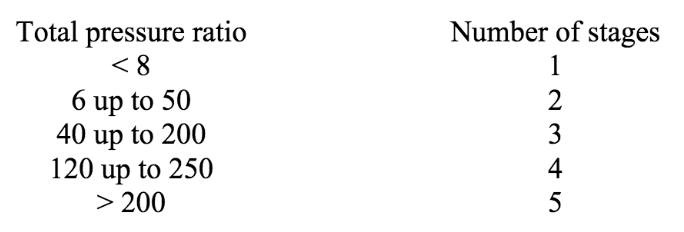
\includegraphics[scale=0.8]{ch5/22}
\captionof{table}{}
\end{center}

We can see that some pressure ratios are situated in 2 stage numbers. One has to choose in function of the use. If we use the compressor everyday continuously, then it is better to invest more at the acquisition to lower the maintenance and consumption costs. If we use it for example once a day, then take the cheapest. 

\section{Centrifugal turbochargers}
\subsection{Introduction}

\minifig{ch5/23}{ch5/24}{0.3}{0.3}{0.49}{0.49}
This is one of the most efficient compression system for high compression ratio. The wheel is mounted on the shaft and on this wheel we have a passage for the flow between blades. On top of that we have a cover. The blades can be purely radial or shifted. Then we enter in the diffuser where we have vanes (2 rows), before going into the volute. This collector can have different shapes. The volume is increasing as shown on the second figure, it is used mainly to change the direction of the air. The distributor is different from the pump because we have something inside, we have vanes in the distributor. These vanes can rotate in some cases. They are called Variable Stator Vane, or Inlet Guide Vane.

\chapter{Radioactivité $\beta$}
\section{Définitions}
On s'intéresse ici à ce qui se passe dans le noyau, c'est-à-dire que le nombre de nucléons ne sera pas modifié. La
différence de masse $m_{neutron}-m_{proton} = 1.3$ MeV implique que le proton instable mais pas le neutron. La 
radioactivité $\beta$ est un processus pù
\begin{itemize}
\item[$\bullet$] Un neutron est converti en proton : $n\to p+e^-+\bar nu$
\item[$\bullet$] Un proton est converti en neutron : $p\to n+e^++ nu$
\end{itemize}\ 

Il faut qu'il y ai conservation du nombre leptonique (0=0+1-1), du moment cinétique et de l'énergie (le spectre
des électrons est continu). Or, ceci n'était pas vrai si un neutron se changeait "juste" en proton ou inversement. 
C'est pour ça que \textsc{Pauli} a émis l'hypothèse de l'existence du \textit{neutrino} en \textit{1931}, une
particule de spin 1/2 (fermion) et de masse presque nulle interagissant peu avec la matière (si peu que la détection
n'a été rendue possible qu'en \textit{1950}).\\

Il y a d'autres processus lié à la radioactivité $\beta$ : la capture électronique ($p+e^-\to n+\nu$), la 
capture positronique ($n+e^++\to p+\bar\nu$) (pas observée) et l'émission de leptons lourds ($\mu, \tau$) mais 
celle-ci ne se déroule pas dans les noyaux (et on n'en parlera pas, cf. le nom du cours).

\section{Transition $\beta$ dans les noyaux}
Ces transitions ne modifient donc pas le nombre total de nucléons. Elle se manifeste (dans ce cours) sous 
trois aspect
\begin{description}
\item[Transition $\beta^-$]  Un neutron est transformé en proton avec émission (conservation de la charge) d'un 
électron et d'un anti-neutrino (conservation du nombre leptonique et de l'énergie. Si on émet une particule il
faut également une antiparticule). Ceci concerne les isotopes \textit{en-dessous} de la vallée de stabilité qui ont
un excès de neutrons.
\begin{equation}
^A_ZX_N \to A_{Z+1}Y_{N-1} + e^- + \bar \nu
\end{equation}
\item[Transition $\beta^+$] Concerne les isotopes \textit{au-dessus} de la vallée de stabilité, ceux-ci ayant un
excédent de proton. Par $\beta^+$, on revient vers celle-ci (parabole de masse)
\begin{equation}
^A_ZX_N \to A_{Z-1}Y_{N+1} + e^+ + \nu
\end{equation}
\item[Capture électronique] Phénomène allant en parallèle avec $\beta^+$ car ils vont souvent ensemble. La différence
est que la capture donne un spectre \textbf{mono}énergétique (comme $\alpha$) car il n'y a que deux particules 
(s'il y en a trois, la répartition de l'énergie entre deux donne un continuum).
\begin{equation}
^A_ZX_N +e^- \to A_{Z-1}Y_{N+1}^*  + \nu
\end{equation}
\end{description}

\subsection{A. Bilans nucléaires}
Nous allons regarder le bilan d'énergie qui sera ici plus compliqué car il faut tenir compte de la différence
de masse du neutron et du proton, mais également que leur nombre change. Notons que les bilans sont ici 
nucléaires (le nuage électronique est négligé).

\subsubsection{Transition $\beta^-$}
Partons d'un état d'initiale avec une certaine masse exprimée avec l'énergie de liaison $B$
\begin{equation}
m(A,Z) = Zm_pc^2 + Nm_nc^2 - B(A,Z)
\end{equation}
Il faut tenir compte des énergies cinétiques pour l'état final 
\begin{equation}
m(A,Z+1) +m_ec^2+T_e+T_\nu = (Z+1)m_c^2+(N-1-m_nc^2-B(A,Z+1)+m_ec^2+T_e+T_\nu
\end{equation}
Par conservation de l'énergie
\begin{equation}
T_e+T_\nu = Q_{\beta^-}^N = B(A,Z+1)-B(A,Z)+\underbrace{(m_n-m_p-m_e)c^2}_{0.782\text{ MeV}}
\end{equation}
La quantité $ Q_{\beta^-}^N$ (seuil) doit être positive afin que la transition soit possible. L'électron et 
le neutrino se partagent l'énergie de seuil donnant un spectre continu (trois corps).


\subsubsection{Transition $\beta^+$}
En suivant un résultat analogue, on trouve pour le seuil
\begin{equation}
Q_{\beta^+}^N = B(A,Z-1)-B(A,Z)-\underbrace{(m_n-m_p-m_e)c^2}_{1.804\text{ MeV}}
\end{equation}
La différence vient du fait que neutron et proton n'ont pas exactement la même masse.


\subsection{Bilans atomiques}
Prenons cette fois-ci en compte les électrons. 

\subsubsection{Transition $\beta^-$}
	\begin{wrapfigure}[9]{r}{7cm}
%	\vspace{-5mm}
	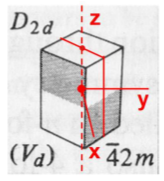
\includegraphics[scale=0.4]{ch6/image1}
	\captionof{figure}{ }
	\end{wrapfigure}

Dans l'état initial, l'atome est neutre : $Z$ protons, $N$ neutrons et $Z$ électrons formant un cortège 
électronique. L'état final est un ion positif : $Z+1$ protons, $N-1$ neutrons et $Z+1$ électrons. Le seuil 
atomique est donné par
\begin{equation}
\begin{array}{ll}
Q_{\beta^-}^a &= M(A,Z)c^ 2 - [M^*(A,Z+1)c^2+m_ec^2]\\ &\approx M(A,Z)c^2+M(A,Z+1)c^2
\end{array}
\end{equation}
où nous avons négligé l'énergie d'ionisation de l'électron.

\newpage
Comparons les deux seuils (atomique et nucléaire)
\begin{equation}
Q_{\beta^-}^a \approx M(A,Z)c^2-M(A,Z+1)c^2,\qquad\qquad
Q_{\beta^-}^N = m(A,Z)-m(A,Z+1)-m_ec^2
\end{equation}
On comparaison avec le seuil nucléaire $M(A,Z)c^2 = m(A,Z)+Zm_e+B_e$. Dès lors, si les énergies de liaison 
$B_e$ sont proches dans les états initial et final, nous avons que $Q_{\beta^-}^a\approx Q_{\beta^-}^N$. Ceci
n'est pas toujours vrai comme le montre le $^{187}$Re (voir \textit{slide 78}).



\subsubsection{Transition $\beta^-$}
	\begin{wrapfigure}[9]{r}{7cm}
%	\vspace{-5mm}
	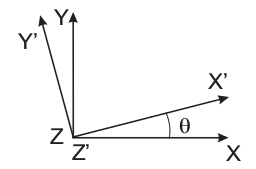
\includegraphics[scale=0.4]{ch6/image2}
	\captionof{figure}{ }
	\end{wrapfigure}
Les signes changent mais l'idée est la même. Dans l'état initial, l'atome est neutre : $Z$ protons, $N$ neutrons 
et $Z$ électrons formant un cortège électronique. L'état final est un ion négatif : $Z-1$ protons, $N+1$ neutrons 
et $Z$ électrons. Le seuil 
atomique est donné par
\begin{equation}
\begin{array}{ll}
Q_{\beta^+}^a &= M(A,Z)c^2 - [M^*(A,Z-1)c^2+m_ec^2]\\ &\approx M(A,Z)c^2+M(A,Z-1)c^2-2m_ec^2
\end{array}
\end{equation}
où nous avons négligé l'énergie d'ionisation de l'électron.

\subsubsection{Capture électronique}
	\begin{wrapfigure}[14]{l}{8.5cm}
	\vspace{-5mm}
	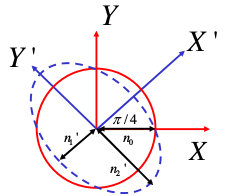
\includegraphics[scale=0.55]{ch6/image3}
	\captionof{figure}{Parabole de masse (gauche $\beta^-$, droite $\beta^+$). Le seuil $Q_{\beta^+}$ n'est
	 pas simplement la différence de masse mais celle différence soustraite de $2m_ec^2$. Cette compétition ne
	 concerne que $\beta^+$. Le seuil différent implique que certaines transitions ne sont que de type CE.}
	\end{wrapfigure}

La capture électronique est un phénomène qui rentre en compétition avec $\beta^+$ où un électron du cortège
électronique est capturé pour former un noyau dans lequel un proton est transformé en neutron. 
\begin{equation}
^A_ZX_N+e^-\to ^A_{Z-1}Y^*_{N+1}+\nu
\end{equation}
où le cortège électronique est excité. Ici les neutrinos sont monoénergétique (ce qui n'est \textbf{pas} le cas
pour la désintégration $\beta^\pm$). Ce phénomène est par contre impossible pour un atome complètement isolé.
Si cela va "ensemble" avec $\beta^+$, c'est parce que le même noyau est produit à partir du même noyau initial. 
La différence importante, ce sont les seuils (différence de masses avec une petite correction $\Delta_{el}$ souvent
négligeable) qui diffèrent de $2m_ec^2$. En effet, le bilan final donne
\begin{equation}
Q_{CE} = M(A,Z)c^2-M(A,Z-1)c^2-\Delta_{el}\approx Q_{\beta^+}^a + 2m_ec^2
\end{equation}
L'électron final fait donc partie du cortège électronique de $\Delta_{el}$ est l'énergie d'excitation de l'atome
$Y$ (proportionnel à l'énergie de liaison de l'électron capturé). Il y a formation d'un "trou" dans le couche
électronique de $Y$ causant une réorganisation du cortège électronique.\\

Considérons le spectre des électrons. Si on néglige l'énergie de recul (l'énergie cinétique du noyau fille $Y$), 
pour $\beta^\pm$ nous avons
\begin{equation}
Q_\beta = T_e+T_\nu
\end{equation}
L'électron et le neutrino se partage l'énergie libérée ce qui fait que l'énergie de l'électron varie de façon
continue de 0 à $Q_\beta$. L'énergie totale libérée vaut donc $E=m_e+Q\beta$. Pour la capture électronique, le
spectre des neutrinos est monoénergétique $Q_{CE} = T_\nu$.

\newpage
\begin{center}
	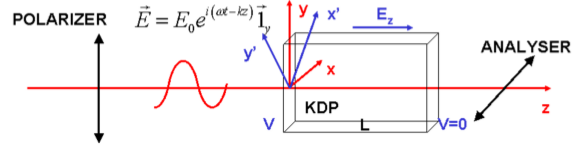
\includegraphics[scale=0.55]{ch6/image4}
	\captionof{figure}{Comme pour $\alpha$, il y a d'autres transitions que vers le fondamental pour autant que 
	les seuils soient respectés. Il y a compétition $\beta^+/CE$ mais la valeur de $2m_ec^2$ fait que l'on peut
	avoir du $\beta^+$ seulement en dessous de ce seuil et au dessus seulement de la capture électronique}
\end{center}\ 

\section{Théorie de Fermi}

\subsection{Généralités}
Cette théorie a été établie (de façon incomplète) en \textit{1934} en se basant sur l'analogie avec l'émission
d'un photon. Afin d'être précis, il y a nécessite de faire des calculs relativistes ($m_\nu\approx0, m_ec^2
\approx 0.511$ MeV). La règle d'or de \textsc{Fermi} permet d'estimer la probabilité de transition d'un état
vers un autre
\begin{equation}
\dfrac{dW}{dE} = \dfrac{2\pi}{\hbar}|V_{fi}|^2\rho(E)
\end{equation}
où $\rho(E) = \frac{dN}{dE_T}$ est la densité de niveaux à l'énergie $E_T=E_e+E_\nu$, d$\rho_\alpha(E) : 
\frac{(4\pi)^2}{(\hbar c)^2}(Q_\beta-T_e)^2k_e(T_e+m_ec^2)dT_e$ et $V_{fi}$ est l'élément de matrice de 
la transition $\beta$ que nous allons maintenant approfondir.

\subsubsection{Élément de matrice de transition $V_{fi}$}
Celui-ci est défini par
\begin{equation}
V_{fi}\equiv \bra{\Psi_f^N\Psi_e}G_FO_\beta\ket{\Psi_i^N\Psi_\nu}
\end{equation}
où $O_\beta$ est un opération de transition sans dimension et $G_F$ la constante de couplage de désintégration
$\beta$ (ou \textit{constante de Fermi}). Elle joue un rôle analogue à $e^2$ pour l'interaction électromagnétique 
(dimension $E\times L^3$). Elle est donnée par
\begin{equation}
G_F = m_ec^2\left(\frac{\hbar}{m_ec}\right)^3G_\beta
\end{equation}
où $G_\beta = 3.002\times 10^{-12}$. On retrouve également quatre fonctions d'ondes
\begin{enumerate}
\item[$\bullet$] $\Psi_i^N$, la fonction d'onde initiale nucléaire
\item[$\bullet$] $\Psi_f^N$, la fonction d'onde finale nucléaire
\item[$\bullet$] $\Psi_\nu$, la fonction d'onde du neutrino (selon la théorie des champ, l'apparition d'une 
antiparticule entraîne la disparition d'une particule)
\item[$\bullet$] $\Psi_e$, la fonction d'onde de l'électron
\end{enumerate}\ 

Pour rendre son traitement plus simple, on va la factoriser en une partie nucléaire et une partie leptonique
\begin{equation}
V_{fi} \approx G_F \bra{\Psi_f^N}O^N_\beta\ket{\Psi_i^N}\bra{\Psi_e}O^L_\beta\ket{\Psi_\nu}
\end{equation}
Pour la partie nucléaire, $M_{fi} = \bra{\Psi_f^N}O^N_\beta\ket{\Psi_i^N}$ doit être calculé à partir de 
modèles nucléaires.\\

La partie leptonique "provient" de l'intérieur du noyau. Comme le noyau est "petit" par rapport aux longueurs 
d'onde de l'électron et du neutrino (soit $\vec{r}$, la coordonnée commune de l'électron et du neutrino), on va
pouvoir faire quelques approximations. La première que que le neutrino n'interagit pas
\begin{equation}
\Psi_\nu \approx e^{i\vec{k}_\nu.\vec{r}}\approx1
\end{equation}
Un raisonnement similaire peut être tenu pour l'électron, mais celui-ci interagit avec les protons. Il faut donc
tenir compte de la fonction d'onde au voisinage de zéro (dépend de la charge du noyau)
\begin{equation}
\Psi_\nu \approx e^{i\vec{k}_e.\vec{r}}\Psi_e(0)\approx\Psi_e(0)
\end{equation}
Évaluons alors l'élément de matrice (via \textsc{Fermi})
\begin{equation}
|\bra{\Psi_e}O^L_\beta\ket{\Psi_\nu}|^2 \propto |\Psi_e(0)|^2|\Psi_\nu(0)|^2 = \frac{1}{(2\pi)^6}F(\pm Z, p_e)
\end{equation}
où l'on voit apparaître la fonction de \textsc{Fermi}, qui dépend de l'énergie (par le paramètre de 
\textsc{Sommerfeld}, $\eta$). Notons la normalisation de l'onde plane
\begin{equation}
\bra{e^{i\vec k.\vec r}}\ket{e^{i\vec k'.\vec r}} = (2\pi)^3\delta(\vec{k}-\vec{k}')
\end{equation}

\subsubsection{Fonction de Fermi}
	\begin{wrapfigure}[14]{l}{10.5cm}
	\vspace{-5mm}
	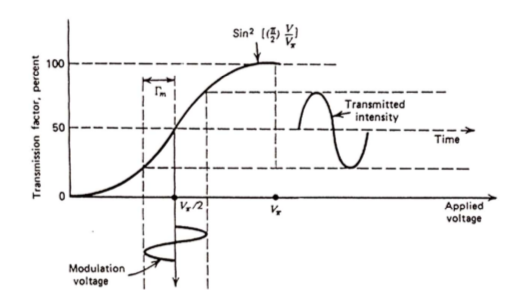
\includegraphics[scale=0.55]{ch6/image5}
	\captionof{figure}{ }
	\end{wrapfigure}
	
Dans un cadre non-relativiste, celle-ci s'écrit
\begin{equation}
F(\pm Z, p_e) : |\Psi_e(0)|^2 = \dfrac{2\pi\eta}{e^{2\pi\eta}-1}
\end{equation}\ \\
\\
\\

Celle-ci est toujours positive et dépend fortement de $Z$.  On y retrouve le \textit{paramètre de Sommerfeld}
qui "mesure" les effets coulombiens
\begin{equation}
\eta = \mp \dfrac{(Z\pm 1)e^2}{\hbar \nu}
\end{equation}
Pour l'émission $\beta^-$, $\eta <0$ et $F>1$, les électrons et le noyau s'attirent alors que pour l'émission
$\beta^+$, $\eta >0$ et $F<1$, les positrons et le noyau se repoussent.


\newpage
\subsubsection{Probabilité de transition totale}
En regroupant tous les différents termes
\begin{equation}
\frac{dW}{dE} = \dfrac{dW}{dT_e} = \frac{1}{2\pi^3}\frac{1}{\hbar(m_ec^2)^4}G_\beta^2cp_e(Q_\beta-T_e)^2(T_e+
m_ec^2)F(\pm Z,p_e)|M_{fi}|^2
\end{equation}
Nous avons bien une factorisation entre une partie purement nucléaire (via $M_{fi}$) et une partie
électronique (la fonction de Fermi dépend à la fois des propriétés électronique et du  noyau et le reste est 
purement électronique). Il existe une relation entre $T_e$ et $p_e$ :
\begin{equation}
E_e = \sqrt{(p_ec)^2+(m_ec^2)^2} = T_e+m_ec^2
\end{equation}

	\begin{wrapfigure}[11]{r}{5.5cm}
	\vspace{-5mm}
	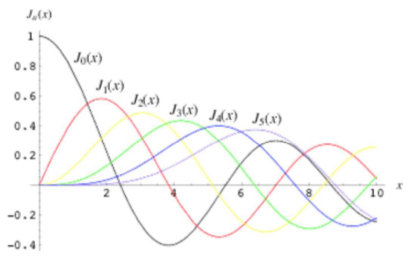
\includegraphics[scale=0.55]{ch6/image6}
	\captionof{figure}{ }
	\end{wrapfigure}
L'expérimentateur va mesurer $dW/dE$. Selon $\beta^\pm$, \textsc{Fermi} va réduire ou augmenter le spectre ce 
qui va causer une différence assez forte entre le spectre $\beta^+$ et le $\beta^-$. En effet $\beta^-$ est 
attiré par le noyau fille et $\beta^+$ repoussé ($T_e=0, F$ très petite).  Les comportement asymptotiques pour
$T_e=0$ sont
\begin{equation}
\beta^+ : F(\pm Z, p_e)\to 0,\qquad\qquad \beta^- : F(\pm Z, p_e)\to \frac{1}{\sqrt{T_e}}
\end{equation}
Notons que $dW/dE$ est non nul pour $T_e=0$. Comme annoncé ci-dessus, le spectre est continu pour des énergies 
entre 0 et $Q_{\beta}$. La durée de vie peut s'obtenir par intégration sur toutes les énergies cinétiques tandis
que la probabilité de transition totale est donnée par l'intégrale sur les énergies: $W = dW/dT_edT_e$ où 
$M_{fi}$ n'interviendra pas dans son calcul, étant un terme purement nucléaire.



\subsubsection{Élément de matrice nucléaire $M_{fi}$}
Celui-ci est défini par
\begin{equation}
|M_{fi}|^2 = B(F)+\lambda^2B(GT)
\end{equation}
On y retrouve la probabilité de transition réduite (elle même défini par deux opérateurs définissant les 
transitions $\beta$)
\begin{equation}
B(\sigma) = \dfrac{2J_f+1}{2J_1+1}|\bra{\Psi^{J_f\pi_f}}O(\sigma)\ket{\Psi^{J_i\pi_i}}|^2
\end{equation}
où $\Psi^{J_{i/f}\pi_{i/f}}$ sont les fonctions d'ondes du noyau dans l'état initial/final. On retrouve
aussi l'\textbf{opérateur de Fermi} $O(F)$ (à admettre)
\begin{equation}
O(F) = \sum_{i=1}^A t_{i,\pm} = T_\pm
\end{equation}
Il s'agit d'un OTI de rang 0 dans l'espace des spin et de rang 1 dans l'espace des isospins. Il ne dépend 
pas de $J$ mais seulement de l'isospin : il ne change pas par rapport au spin du noyau.\\

On trouve de même l\textbf{opérateur de Gamow-Teller} $O(GT)$
\begin{equation}
O(GT) = \sum_{i=1}^A \sigma_i t_{i,\pm}
\end{equation}
Qui est un OTI de rang 1 dans l'espace des spin et des isospin.\\

Les signes $\pm$ ci dessus signifient : + pour la radioactivité $\beta^+$ ($t_{i+}$ change un proton en un 
neutron) et - pour la radioactivité $\beta^-$ ($t_{i-}$ change un neutron en un proton).


\section{Règles de sélection}
\subsection{Transition de Fermi}
L'opérateur ne dépend pas du spin, il n'y a pas besoin de \textsc{Wigner-Eckaert}. Le spin initial doit
être le même que le spin final : $J_i=J_f$. Il ne dépend pas non plus de la parité, il doit être invariant
par réflexion (pair) : $\pi_i=\pi_f$. Il s'agit par contre d'un OTI de rang 1 dans l'espace des isospin. 
Regardons l'élément de matrice :
\begin{equation}
\bra{T'M_T'}T_\pm\ket{TM_T} = \sqrt{(T\mp M_T)(T\pm M_T+1)}\delta_{TT'}\delta(M_T'M_{T\pm1}
\end{equation}
Il faut que les $T$ soient identiques. De plus, l'opérateur $T_\pm$ change la projection (augmente ou diminue) 
mais pas la valeur du moment cinétique (isospin). En résumé
\begin{equation}
J_i=J_f,\qquad\qquad \pi_i=\pi_f,\qquad\qquad T_i=T_f
\end{equation}


\subsection{Transition de Gamow-Teller}
Cet opérateur est invariant par réflexion. l s'agit d'un OTI de rang 1 dans l'espace des spin mais aussi dans
celui des isospin. Il faut que
\begin{equation}
|J_i-J_f| \leq 1 \leq J_i+J_f,\qquad\qquad \pi_i=\pi_f, \qquad\qquad |T_i-T_f| \leq 1 \leq T_i+T_f
\end{equation}\ \\
\\
Afin d'avoir des transition de \textsc{Fermi} et \textsc{Gamow-Teller}, il faut que
\begin{equation}
J_i=J_f\neq 0,\qquad\qquad \pi_i=\pi_f,\qquad\qquad T_i=T_f\neq 0
\end{equation}

\begin{center}
	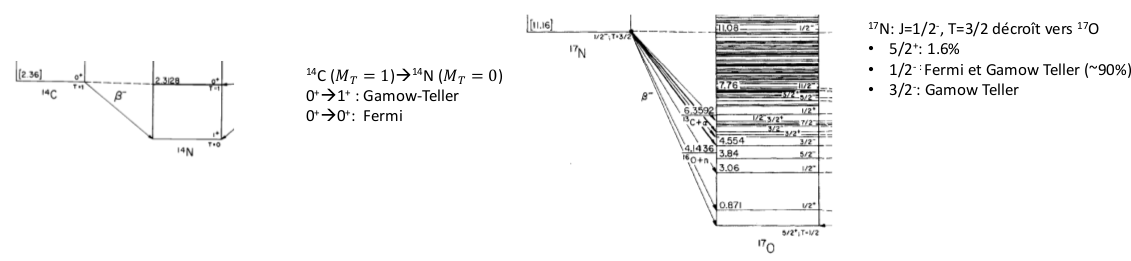
\includegraphics[scale=0.4]{ch6/image7}
	\captionof{figure}{A gauche ; deux transitions sont autorisée (soit purement l'une, soit purement l'autre). A
	droite ; plus compliqué à cause d'une grande densité de niveau.}
\end{center}



\subsection{Transition interdite}
Si les deux conditions ne sont pas satisfaites, il faut reconsidérer les précédentes approximations. Pour se faire,
partons de l'onde plane de l'électron
\begin{equation}
e^{i\vec k_e.\vec r} \approx \underbrace{1}_{1}+ \underbrace{i\vec{k_e}.\vec{r}}_{2}+
\underbrace{\frac{1}{2}(i\vec{k_e}.\vec{r})^2}_{3} + \dots
\end{equation}
\begin{enumerate}
\item Transition permise
\item Transition une fois interdite : $\pi_i\pi_f=-1, \Delta J = 0,\pm1, \pm2$
\item Transition deux fois interdite : $\pi_i\pi_f=+1, \Delta J = 0,\pm1, \pm2, \pm3$
\end{enumerate}\ 

Si les deux premiers sont interdits, il faut prendre le troisième et ainsi de suite. Chaque terme additionnel est
de plus en plus petit mais il faut en tenir compte car les dominants ne contribuent pas. Il existe un cas
extrêmement pathologique du $^{115}_{49}In(9/2^+)\to ^{115}_{50}Sn(1/2^+)$ où les quatre premiers termes sont
interdits. La probabilité de transition est donc très faible ce qui lui confère une longue durée de vie
($4.4\times 10^{14}$ ans).



\section{Probabilité de transition intégrée}
L'intégration de 
\begin{equation}
\frac{dW}{dE} = \dfrac{dW}{dT_e} = \frac{1}{2\pi^3}\frac{1}{\hbar(m_ec^2)^4}G_\beta^2cp_e(Q_\beta-T_e)^2(T_e+
m_ec^2)F(\pm Z,p_e)|M_{fi}|^2
\end{equation}
sur toutes les énergies électroniques donne la probabilité de transition intégrée. Celle-ci vaut
\begin{equation}
W = \frac{1}{2\pi^3}\frac{m_ec^2}{\hbar}G_\beta^2f(Q_{\beta},\pm Z)|M_{fi}|^2
\end{equation}
où $\DS f(Q_\beta, \pm Z) = \frac{c}{(m_ec^2)^5}\int_0^{Q_\beta} p_e(Q_\beta-T_e)^2(T_e+m_ec^2)F(\pm Z, p_e)dT_e$.\\


	\begin{wrapfigure}[9]{r}{6cm}
	\vspace{-8mm}
	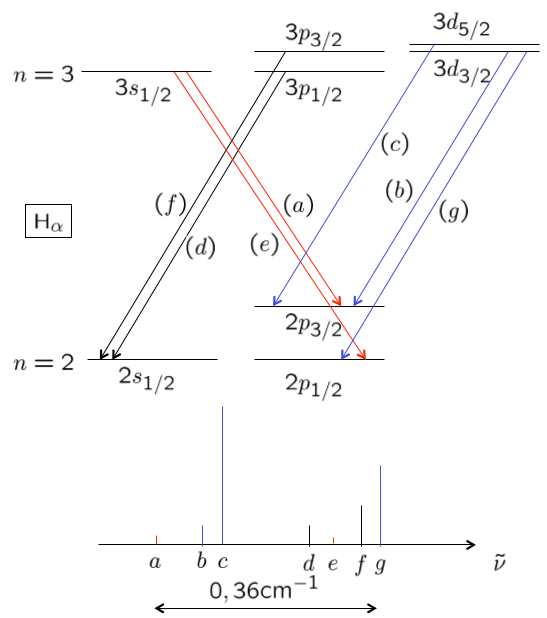
\includegraphics[scale=0.45]{ch6/image8}
	\captionof{figure}{ }
	\end{wrapfigure}
Il s'agit de l'\textit{intégrale de Fermi} (sans dimension). La dépendance en $Q_\beta$ est forte car le seuil 
est petit : peu d'énergie pour l'électron et le neutrino. On parle d'\textit{espace de phase}, soit l'ensemble des
états dans lequel on peut trouver le neutrino et l'électron. Forcément si $Q_\beta$ est petit, l'espace des phases
est petit et la probabilité de transition est petite (à gauche). Les durées de vie sont donc très variables et
il y a une différences entre $\beta^+$ et $\beta^-$.\\

Sachant que la demi-vie est donnée par $t_{1/2} = \ln 2/W$, on peut en déduire la valeur de $ft$
\begin{equation}
ft_{1/2} = \ln2\dfrac{2\pi^3\hbar}{m_ec^2G_\beta^2|M_{fi}|^2}
\end{equation}
Le temps de demi-vie à les dimension d'un temps, il est indépendant de $Q_\beta$ et ne dépend que de l'élément de
matrice nucléaire $M_{fi}$. Il se peut que $t_{1/2}$ varie de plusieurs ordre de grandeur. Si $\log_{10} ft_{1/2}$
vaut 3-6 la transition est permise, si 6-9 une fois interdite et si elle vaut 22.5 elle est quatre fois 
interdites.\\

Etudions le cas particulier d'une \textbf{transition entre deux états d'un même multiplet d'isospin}. Les parties
spatiales doivent être similaires ($M_{fi}$ maximum, transitions \textit{superpersmises}).  Considérons le 
cas très simple d'une transition $\beta^+$ où $J_i=0^+, T_i=1, M_{Ti}=-1, J_f=0^+, T_f=1,M_{Tf}=0$. Les 
transition de \textsc{Gamow-Teller} sont interdites ($J_i=J_f=0$), seulement \textsc{Fermi}. L'élément de matrice
nucléaire $|M_{fi}|^2\approx 2$ de sorte que $\log_10(ft)\approx 3$ (ordre de 3000s).

\newpage
\begin{center}
	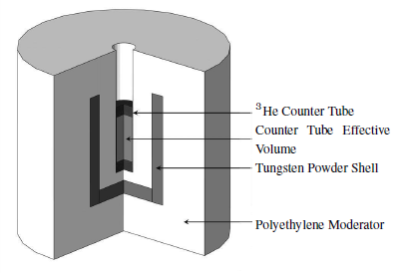
\includegraphics[scale=0.5]{ch6/image9}
	\captionof{figure}{Trois cas différent, trois état avec un même multiplet : les valeurs de $ft_{1/2}$ sont 
	comparables. Les durées de vies sont relativement différentes mais ça c'est à cause de la fonction $f$, 
	différentes dans chacun des cas.}
\end{center}








\section{Capture électronique}
\section{Autres processus}


%%%%%%%%%%%%%%%%%
% Bibliographie %
%%%%%%%%%%%%%%%%%
%\newpage
%\chapter{Bibliographie}
%\nocite{*}
%\printbibliography[heading=none]

%%%%%%%%%%%
% Annexes %
%%%%%%%%%%%
\appendix
%\input{annexes/annexe1.tex}


\end{document}
